% chktex-file 1,3,36,44
\documentclass{ctexbook}

\usepackage{silence}
\usepackage[top=2cm, bottom=2cm, left=2.5cm, right=2.5cm]{geometry}
\usepackage{graphicx}
\usepackage{grffile}
\graphicspath{{D:/code/Math_behind_Signal_and_System/Figures}}
\usepackage{amsmath,amssymb,amsfonts}
\usepackage{dsfont}
\usepackage{hyperref}
\usepackage{fix-cm}
\usepackage{bm}
\usepackage{xcolor}
\usepackage{array}
\usepackage{booktabs}
\usepackage{float}
\usepackage{pifont}
\usepackage{enumitem}
\usepackage{tikz}
\usepackage{hyperref}
\usetikzlibrary{shapes,arrows,positioning,calc}
\usepackage{silence}
\WarningFilter{latex}{Font shape}
\WarningFilter{latex}{Some font shapes}
\WarningFilter{latex}{Underfull \vbox}
\WarningFilter{latex}{Underfull \hbox}
\vfuzz=100pt  % 垂直方向容忍度
\hfuzz=100pt  % 水平方向容忍度  
\vbadness=10000
\hbadness=10000
\overfullrule=0pt  % 不标记过满行

\WarningFilter{hyperref}{Token not allowed in a PDF string}
\allowdisplaybreaks[1]
\raggedbottom

\newcommand{\shah}{\operatorname{III}}
% 便捷命令:在文中书写原函数在上下限的取值,例如 \evalat{F(x)}{a}{b} 输出为 \left.F(x)\right|_{a}^{b}
\newcommand{\evalat}[3]{\left.#1\right|_{#2}^{#3}}
\NewDocumentCommand{\lr}{m m}{%
  \par\nopagebreak
  \noindent%
  \makebox[\textwidth][c]{%
    $\displaystyle
    \color{blue}\begin{aligned}#1\end{aligned}$%
    \hspace{1em}%
    \vrule
    \hspace{1em}%
    $\displaystyle
    \color{red}\begin{aligned}#2\end{aligned}$%
  }%
  \par\nopagebreak
}
\newlist{circlist}{enumerate}{1}
\setlist[circlist]{
    label=\protect\ding{\numexpr171+\arabic*\relax},
    left=0pt
}


\title{信号与系统的数学基础}
\author{Math behind Siganal and Sysdem}
\date{\today}
\begin{document}

\maketitle{}%封面
\frontmatter%前言
信号与系统是电子信息等相关专业本科生的重要基础课,是后续课程“数字信号处
理”“通信原理”“自动控制”“随机信号处理”“数字图像处理”“现代信号处理”等课程的基
础,以确定信号通过线性时不变系统的过程为核心,综合运用多门数学课程的知识,尤
其是傅里叶分析。

然而,国内外的信号与系统课程对于傅里叶级数、傅里叶变换和拉普拉斯变换的定
义有所不同,国内的课程中所谓“频域分析”实际上指的是角频率域,而这种定义上的不
同会导致诸多公式的内核相同但形式不同,使学习者感到困惑。我自学过斯坦福大学
公开课EE261,同样面临着这个问题,所以希望尝试这种新的笔记形式,梳理信号与系
统课程的理论部分,同时也使本书能够作为同学们学习信号与系统时的参考书。同时,
我注意到现在的信号与系统教材中对很多数学上的内容的处理过于简单化,以至于同学
们对一些公式感到不解,我希望结合《信号与系统》教材和一些数学专业的实变函数、
傅里叶分析教材,对这样的内容做一些简单的补充和深化。

本书将不会涉及信号与系统实践部分,对一些语文性质的概念从简处理,希望了解这些
内容的读者可以自行查看信号与系统教材;对于两种不同的傅里叶变换,将并排给出两
种公式,左侧为频率版本,右侧为角频率版本;此外,为了逻辑的完整性和内容的精确
性,本书会引入一些对工科生较难理解的内容,对于勒贝格积分,读者应当明白其大体
思想,技术细节则不在我们关注的范围,对于另外一些内容,将用“*”标注或直接用语
言声明,读者可以自行选择是否阅读这些内容。

限于作者水平,书中难免存在不足之处,希望读者可以提出宝贵的意见或建议,可以反
馈至我的电子邮箱:2024212622@bupt.cn。

{
\raggedleft{}
北京市十一学校2024届毕业生\\
严子竣\\
2025年秋\\
}
\tableofcontents%目录
\mainmatter%正文
\chapter{信号与系统概述}%第一章
\section{信号与系统的基本概念}
信号 (signal)是信息 (information)的表现形式与传送载体,信息是蕴含在信
号中的具体内容。

在电学领域中,通过电压或电流对真是信号进行连续的记录,模拟其变化过程得到
的信号称为模拟信号 (analog signal)或连续信号 (continuous signal),但由于
计算机中信号只能以有限位数的形式储存,往往需要将模拟信号转化为数字信号
(digital siganal)。这个过程往往需要利用模数转换器 (analog-to-digital converter,ADC)
,使用时再利用数模转换器 (digital-to-analog converter,DAC)将数字信号转化
为模拟信号。

在信息科学与技术领域,系统指对信号产生影响的装置或算法,例如滤波系统、调制系
统、发射系统,将这些系统组合起来就组成了无线电广播系统;例如通信系统由信源、
发射机、信道、接收机和信宿五个部分组成。

\section{连续信号与离散信号}\label{sec:signal}
信号的本质是函数,\textbf{连续信号}就是定义域“连续”的函数,例如一个时间的函数$f(t)$,
一般要求定义域具有连续统的势。相应的,\textbf{离散信号}的定义域往往是至多可数集,于是
我们常认为其定义域是整数集,并记离散信号为$x[n]$,用研究数列的方法研究离散信
号。

从电学的经验来看,电压、电流信号的功率总为其幅值的平方乘以某个常数,于是对于
一般的信号我们也采取此定义。真实的物理世界中的信号的能量总是有限的,但是,为
了更好地研究它们,很多时候使用真实信号的一部分做适当延拓作为研究对象,因此课
程中将遇到一些不满足“方均可积”性质$\int_{-\infty}^{\infty}| f(x)| ^2\,dx
    <\infty$的信号,我们将这种信号称为\textbf{功率信号},因其能量无限而功率有限,
而能量有限的信号就称为\textbf{能量信号}。为了区分某段时间内和全时域上的能量和功率,
又将$(-T/2,T/2)$内的能量
\[E_T=\int_{-T/2}^{T/2}| f(x)| ^2\,dx\]
称为\textbf{归一化能量},功率
\[P_T=\frac{1}{T}\int_{-T/2}^{T/2}| f(x)| ^2\,dx\]
称为\textbf{归一化功率};
\[E=\int_{-\infty}^{\infty}| f(x)| ^2\,dx\]称为\textbf{全时域能量},
\[P=\lim_{T \to \infty}  \frac{1}{T}\int_{-T/2}^{T/2}| f(x)| ^2\,dx\]
称为\textbf{全时域功率}。

类似地,对于离散信号,定义\textbf{归一化能量}为\[E_k=\sum_{n = -k}^{k}  |x[n]|^2\]
\textbf{归一化功率}为\[P_k=\frac{1}{2k+1}\sum_{n = -k}^{k}  |x[n]|^2\]\textbf{全时域能
    量}为\[\sum_{n = -\infty}^{\infty}  |x[n]|^2\]\textbf{全时域功率}为
\[\lim_{k \to \infty}  \frac{1}{2k+1}\sum_{n = -k}^{k}  |x[n]|^2\]

读者可能已经注意到,并不是所有的函数都是可积的,例如$e^x$即使视为功率信号,其
能量和功率也不具有意义,因此它既不属于能量信号,也不属于功率信号;哪怕这个积分
不是反常积分,如狄利克雷函数
\[D(x)=
    \begin{cases}
        1 & x \in \mathbb{Q}    \\
        0 & x \in \mathbb{Q} ^C
    \end{cases}\]
(其中$\mathbb{Q}$ 表示有理数集,上标C在不引起歧义的前提下用来表示取补集)在
黎曼积分(也就是数学分析或高等数学课程,以及多数工科课程中用的积分)的意义下
是不可积的,因为它在所有点不连续,但是这样的函数在\textbf{勒贝格积分}的意义下可积,读
者可以这样理解:勒贝格积分考察函数在某个值处的“区间长度”(严格来讲应为测度)
,狄利克雷函数在一个有限区间上取值1的长度为0,因为有理数是可数集,取值0的长度
就是区间长度,所以其积分值为0。勒贝格积分是黎曼积分的推广,对于非反常积分,黎曼可积的函数一定
是勒贝格可积的,并且在同样的区间上积分值相等。对于勒贝格不可积的函数,一般不
在本课程的讨论范围。尽管我们很少接触只在勒贝格意义下才可积的函数,但后面我们将
逐步认识到勒贝格积分在傅里叶分析中的重要地位,读者应当对其有一个初步的认识。

\section{典型的连续与离散信号}
\noindent 1.\textbf{取样信号}\[Sa(t)=\frac{\sin(t)}{t}\]
它在0处连续延拓为1,在$\pi$的整数倍处为0,是偶函数,在正半轴上的积分值为$\pi /2$(这个结果称为狄利克雷积分)。
国外教材中取样信号一般为一个类似的信号\[sinc(t)=\frac{\sin(\pi t)}{\pi t}=Sa(\pi t)\]
它们的参数不同但性质类似、本质相同,其作用在后续学习采样和插值时将体现出来。需
要注意的是,在绘图时python和MATLAB中只有sinc信号,而且实际上指的是Sa信号。

\noindent 2.\textbf{钟形信号(高斯函数})\[f(t)=Ee^{-{\left(\frac{t}{\tau }\right)}^2}\]
$\tau$为衰减速率或时间常数,$\tau$越大,函数值衰减越慢。

\noindent 3.\textbf{单位脉冲函数/狄拉克函数} (dirac function)
$\delta (x)=\begin{cases}
        0      & x\neq 0 \\
        \infty & x=0
    \end{cases}$可视为一些性质较好的函数如高斯函数、取样函数集中到x=0附近时
的极限情况,从而具备很多优美的性质,见\ref{sec:convolution}。实际上,它还是无限
阶可导的,我们将在\ref{sec:distributions}
中详细讨论这一点。一些简单的性质列举如下。\\
\ding{172} 取样性质:$f(x)\delta (x)=f(0)\delta (x)$\\
\ding{173} 积分性质:$\int_{-\infty}^{\infty}\delta (x)\,dx=1$ (由此我们
说这个函数的强度为1 ),从而
$\int_{-\infty}^{\infty}f(x)\delta (x)\,dx=f(0)$。
\ding{174} $\delta$ 函数是偶函数:$\delta (-x)=\delta (x)$
\ding{175} 尺度变换性质:用函数逼近的观点来理解$\delta $函数,为保证强
度为1,自然应当要求$\delta (ax)=\frac{1}{|a|}\delta (x)$\\
这个函数在做卷积运算时有很好的性质,见\ref{sec:convolution}卷积;关于它的逼近方式,见\\
附录\ref{sec:approach}。我们规定,$\delta_a(x)=\delta (x-a)$,即在$x=a$处取样的狄拉克函数。

\noindent 4.\textbf{单位阶跃函数} (the unit step/Heaviside function)$u(x)=
    \begin{cases}
        0 & x<0 \\
        1 & x>0
    \end{cases}$\\
在0处的值可以任意定义,一般取0、1或1/2,不会有影响,所以一般也不会讨论。由单
位阶跃函数衍生出许多其他函数:\\
\textbf{符号函数}\[sgn(x)=\begin{cases}
        -1 & x<0 \\
        1  & x>0
    \end{cases}=u(t)-u(-t)\]
\textbf{矩形脉冲}\[R_T(t)=u(t)-u(t-T)\]
\textbf{门函数(矩形函数、$\Pi $函数)}\[G_T(t)=\Pi_T(t)=u(t+T/2)-u(t-T/2)\]
这里T为脉冲宽度,不加角标时,默认为1。

单位阶跃函数的积分为单位斜变信号 (the unit ramp),导数为狄拉克函数,从直观上
这不难理解,将在\ref{sec:distributions}中讨论。
\begin{figure}[htbp]
    \centering
    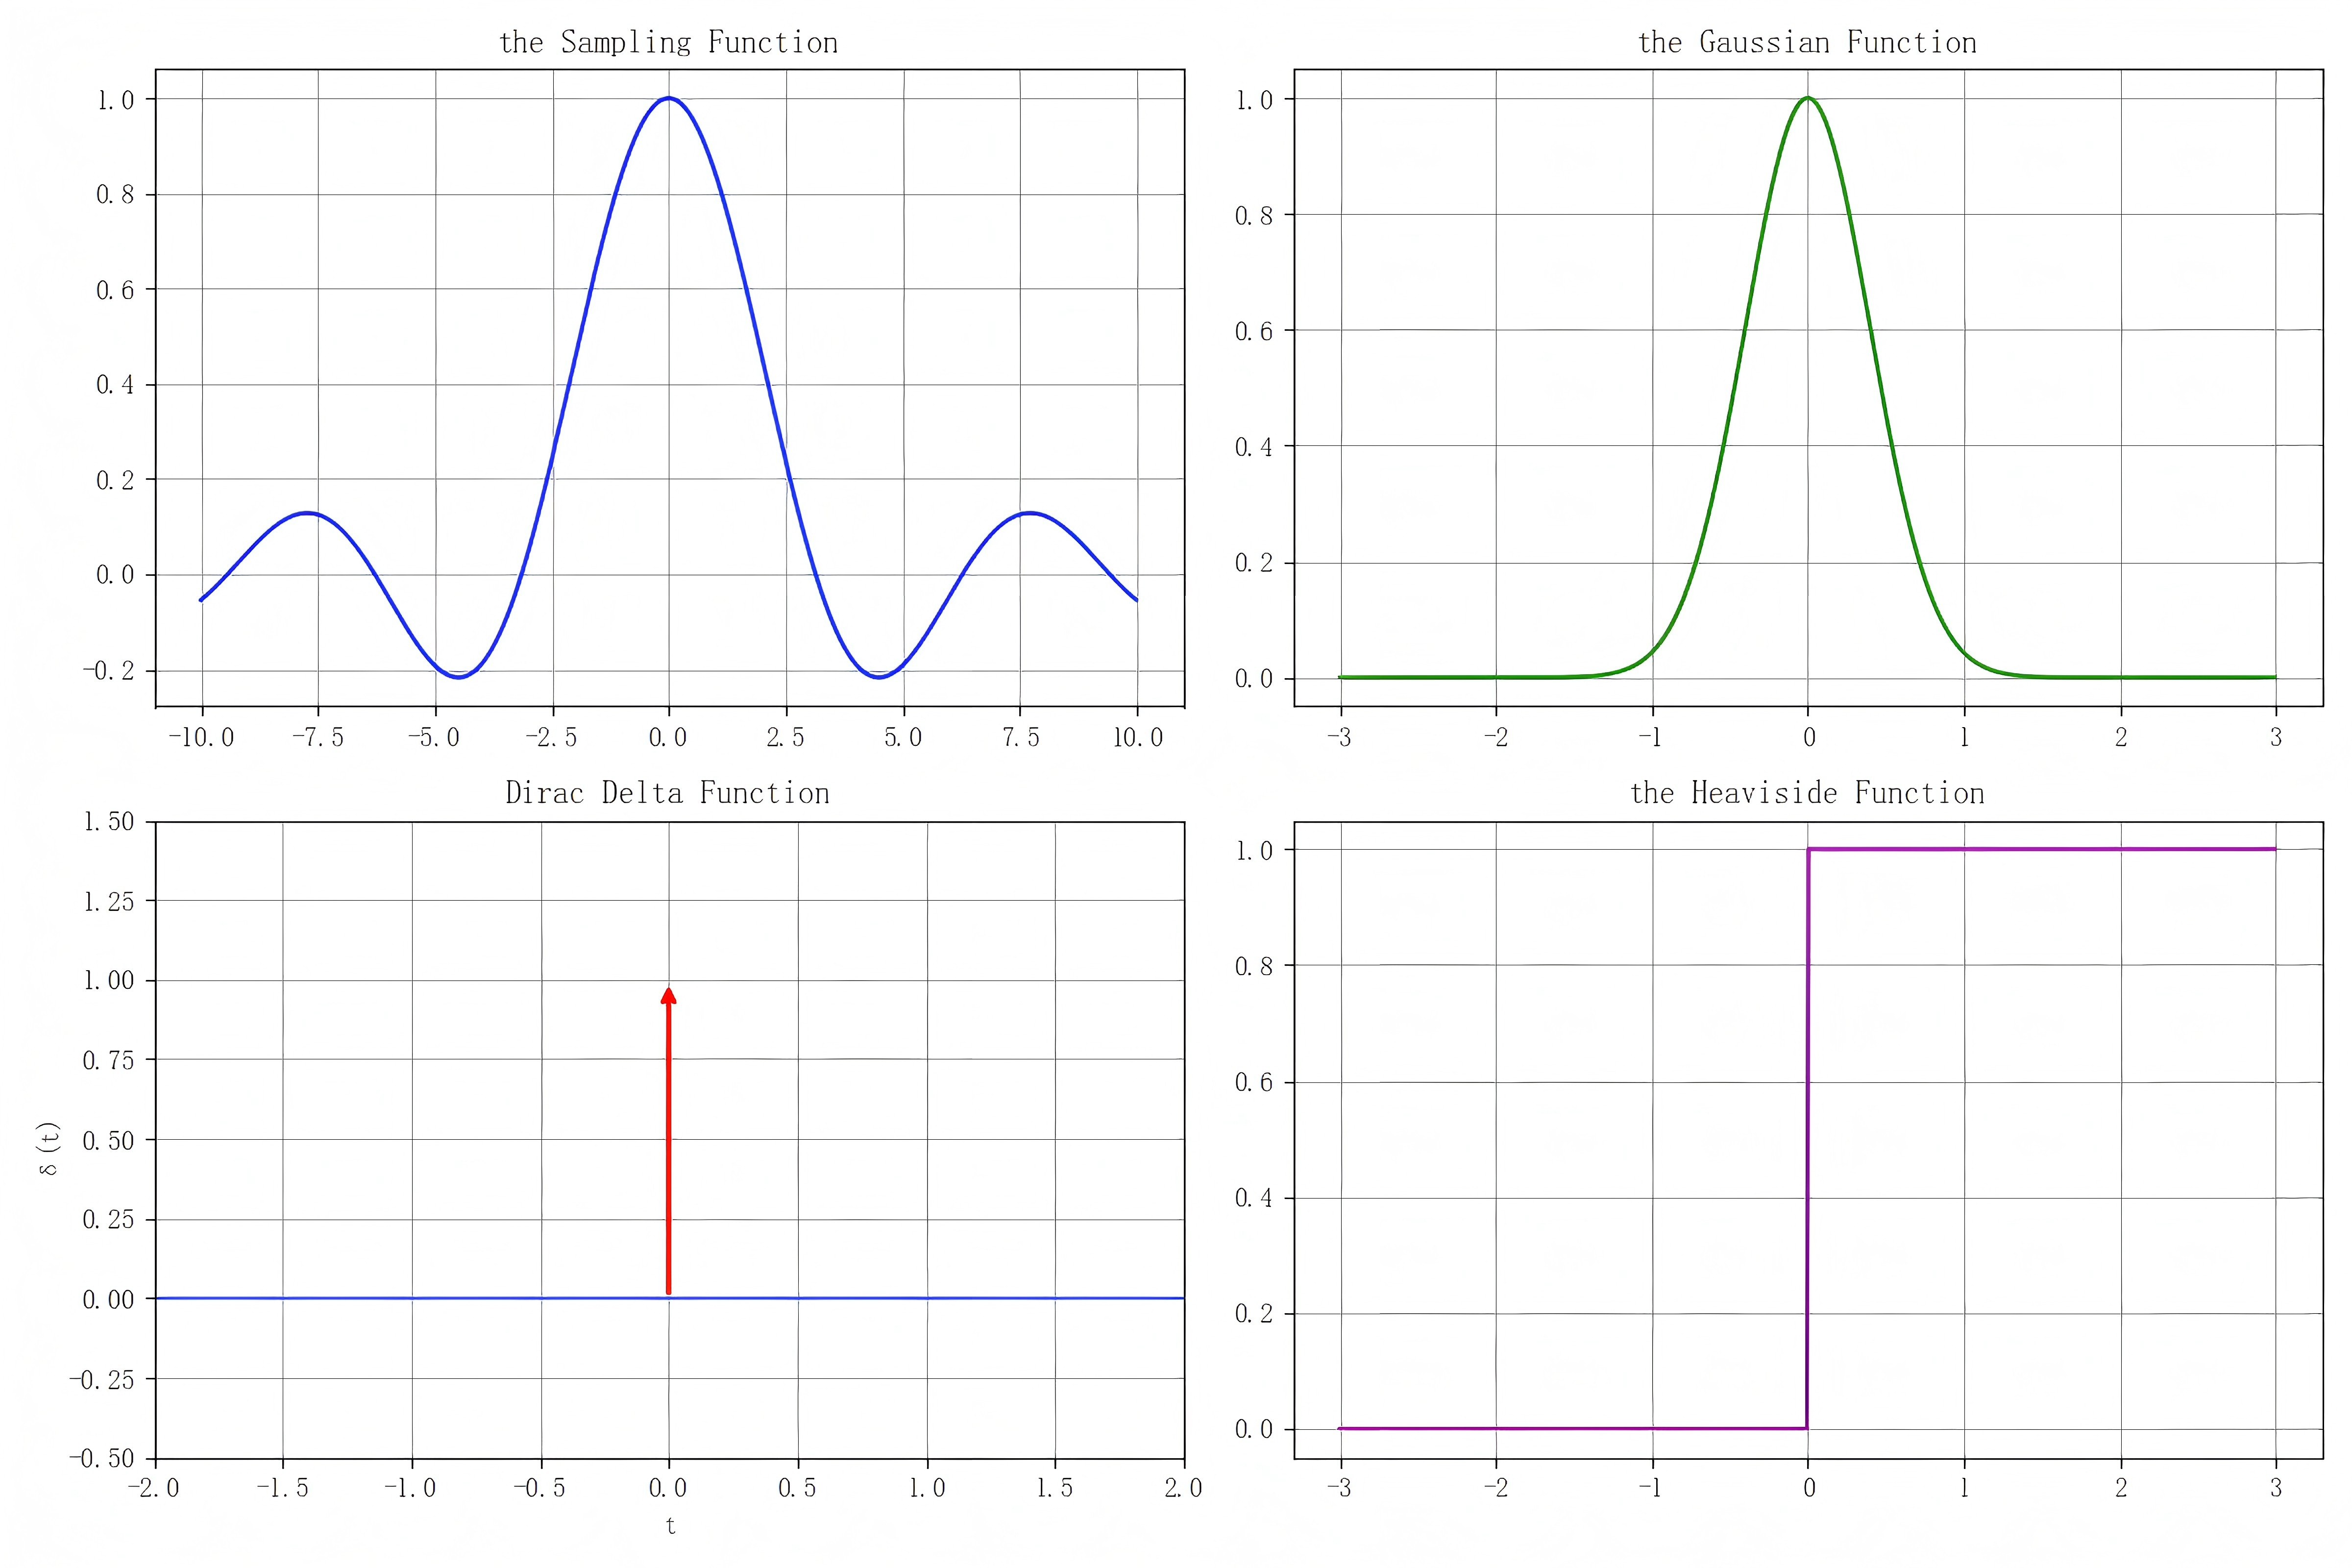
\includegraphics[width=0.7\textwidth]{Figure_1}
    \caption{取样函数、高斯函数、狄拉克函数、单位阶跃函数}
\end{figure}

下面介绍离散信号。\\
1.单位脉冲序列/克罗内克(Kroneker)$\delta$函数
\[\delta[n]=\begin{cases}
        1, & \text{if }n=0     \\
        0, & \text{if }n\neq 0
    \end{cases}\]
将它进行时移,可得\[\delta_k[n]=\delta[n-k]=\begin{cases}
        1, & \text{if }n=0     \\
        0, & \text{if }n\neq 0
    \end{cases}\]
它与狄拉克$\delta$函数一样,都具有取样性质:$x[n]\delta_k[n]=x[k]\delta_k[n],\forall n$.

\noindent 2.单位阶跃序列\[u[n]=\begin{cases}
        1, & \text{if }n\geq 0 \\
        0, & \text{if }n< 0
    \end{cases}\]
类似连续信号,由它可以衍生出矩形窗序列:
\[R_N[n]=n[n]-u[n-N]=\begin{cases}
        1, & \text{if }0\leq n\leq N-1 \\
        0, & \text{otherwise}
    \end{cases}\]

\noindent 3.正弦序列$x[n]=\sin(\Omega_0n)$,其中$\Omega_0$称为数字角频率。
其特点放在以后介绍。
\begin{figure}[htbp]
    \centering
    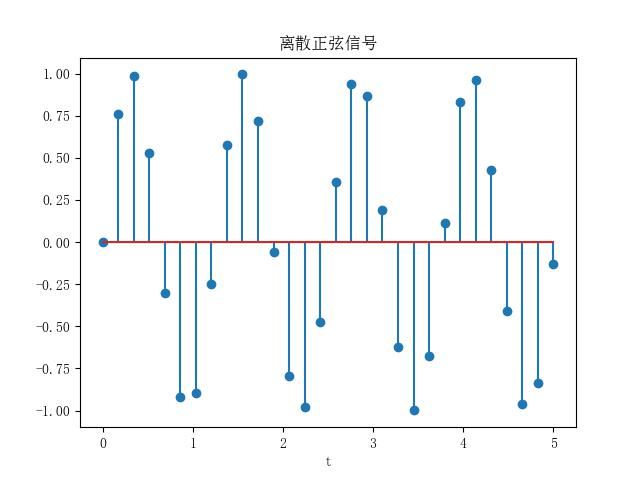
\includegraphics[width=0.5\textwidth]{disct_sin}
    \caption{正弦序列}
\end{figure}

\chapter{连续信号的频域分析}%第二章
在数学分析课程中,我们都学习过傅里叶级数的计算,所以本书将直接回顾几种情况下的
傅里叶级数展开公式,然后从正交函数系的观点出发构建傅里叶级数的理论,再从傅里
叶级数过渡到傅里叶变换,从对周期现象的研究转向对非周期现象的研究,介绍其运算性
质、卷积性质,最后介绍分布(也即广义函数)理论,从而研究常函数、狄拉克函数、正
余弦函数等在常规意义下无法进行傅里叶变换,却又十分重要的函数。

\section{线性空间,正交基}\label{sec:Linear_Space}
首先介绍一些本章需可能用到的概念:度量公理、范数公理、内积公理、正交基、无穷维线
性空间和$L^p$空间,对其不感兴趣的读者,可以等需要时再阅读此小节的内
容,只要知道函数空间上的正交基是怎么回事即可。

在$\mathbb{C}$ -线性空间V中,如果定义了运算
$d(\cdot,\cdot):V\times V\rightarrow \mathbb{C}  $,满足\textbf{度量公理}:
\begin{enumerate}
    \item \textbf{非负性}:$d(x, y) \geq 0$
    \item \textbf{同一性}:$d(x, y) = 0$ 当且仅当 $x = y$
    \item \textbf{对称性}:$d(x, y) = d(y, x)$
    \item \textbf{三角不等式}:$d(x, z) \leq d(x, y) + d(y, z)$
\end{enumerate}
则称在V上定义了一种度量(事实上度量空间不仅能够在线性空间中定义,在一般的拓扑空
间中都能够定义)。

如果定义了运算
$\|\cdot \| :V\rightarrow \mathbb{C} $,满足\textbf{范数公理}
\begin{enumerate}
    \item \textbf{非负性}:$\|\mathbf{x}\| \geq 0$
    \item \textbf{同一性}:$\|\mathbf{x}\| = 0$ 当且仅当 $\mathbf{x} = \mathbf{0}$
    \item \textbf{齐次性}:$\|\alpha \mathbf{x}\| = |\alpha| \, \|\mathbf{x}\|$
    \item \textbf{三角不等式/次可加性}:$\|\mathbf{x} + \mathbf{y}\| \leq \|\mathbf{x}\| + \|\mathbf{y}\|$
\end{enumerate}
则称在V上定义了一种范数,称V为线性赋范空间,又称巴拿赫空间在线性赋范空间上可以定义极限:
\[\lim_{x \to x_0} f(x)=A:=\forall \epsilon>0\exists \delta>0(|x-x_0|<\delta\Rightarrow |f(x)-f(x_0)|<\epsilon) \]
这就是数学分析中的极限定义,只是将绝对值改成了范数,其余类似的极限定义不再赘述。

如果定义了运算
$\langle \cdot,\cdot\rangle:V\times V\rightarrow \mathbb{C} $,满足\textbf{内积公理}
\begin{enumerate}
    \item \textbf{正定性}:$\langle \mathbf{v}, \mathbf{v} \rangle \geq 0$ 且 $\langle \mathbf{v}, \mathbf{v} \rangle = 0$ 当且仅当 $\mathbf{v} = \mathbf{0}$
    \item \textbf{共轭对称性}:$\langle \mathbf{v}, \mathbf{w} \rangle = \overline{\langle \mathbf{w}, \mathbf{v} \rangle}$
    \item \textbf{第一变元的线性性}:
          \begin{itemize}
              \item \textbf{齐性}:$\langle \alpha \mathbf{v}, \mathbf{w} \rangle = \alpha \langle \mathbf{v}, \mathbf{w} \rangle$
              \item \textbf{可加性}:$\langle \mathbf{v} + \mathbf{w}, \mathbf{u} \rangle = \langle \mathbf{v}, \mathbf{u} \rangle + \langle \mathbf{w}, \mathbf{u} \rangle$
          \end{itemize}
\end{enumerate}
则称在V上定义了一种内积 (inner product),称V为内积空间。在内积空间上有著名的
柯西-施瓦兹不等式 (Cauchy-Shwartz inequality):
\[|\langle \mathbf{a,b}\rangle| \leq \| \mathbf{a}\| \| \mathbf{b}\| \]
它有一个经典的证明方法:不妨设$\mathbf{b}$不是零向量,任取$t\in \mathbb{R}$,有
\[0\leq \|\mathbf{a}+t\mathbf{b}\|^2=\|\mathbf{a}\|^2+2t\langle\mathbf{a,b}\rangle +t^2\|\mathbf{b}\|^2\]
令$t=-\frac{\langle\mathbf{a,b}\rangle}{\|\mathbf{b}\|^2}$,即得
\[0\leq \|\mathbf{a}\|^2-2\frac{\langle\mathbf{a,b}\rangle^2}{\|\mathbf{b}\|^2} +\frac{\langle\mathbf{a,b}\rangle^2}{\|\mathbf{b}\|^4}\|\mathbf{b}\|^2=\|\mathbf{a}\|^2-\frac{\langle\mathbf{a,b}\rangle^2}{\|\mathbf{b}\|^2}\]
这与要证明的不等式是等价的。有了柯西-施瓦兹不等式,三角不等式就是显然的了,这里
仅给出其表述,读者可以自行证明:
\[\forall \mathbf{a,b}\in V,\|\mathbf{a+b}\|\leq\|\mathbf{a}\|+\|\mathbf{b}\|\]

不难发现,只要取
$\|\mathbf{v}\|^2=\langle \mathbf{v}, \mathbf{v} \rangle$,
就由内积导出了一种范数,并且这种范数具有比一般的范数更强的性质;
只要取$d(\mathbf{x},\mathbf{y})=\|\mathbf{x-y}\|$,就由范数导出了一种度量,
并且这种度量具有比一般的度量更强的性质。

\textbf{正交基} (othorgnal bases)指的是内积空间V的一组基$\{\mathbf{v_1},\mathbf{v_2},\dots ,\mathbf{v_n}\}$
,满足$\langle \mathbf{v_i},\mathbf{v_j}\rangle =0,i \neq j$ ,对V中任一向量$\mathbf{w}$,
\[\mathbf{w}=\sum_{i = 1}^{n}  c_i \mathbf{v_i}\]
等式两边同时对$\mathbf{v_j}$做内积,得到
\begin{align}
    \langle \mathbf{w},\mathbf{v_j} \rangle=\langle \mathbf{v_j},\sum_{i = 1}^{n}  c_i \mathbf{v_i} \rangle =c_j\langle \mathbf{v_j},\mathbf{v_j} \rangle \\
    c_j=\frac{\langle \mathbf{w},\mathbf{v_j} \rangle}{\langle \mathbf{v_j},\mathbf{v_j} \rangle},
    \mathbf{w}=\sum_{j = 1}^{n}  \frac{\langle \mathbf{w},\mathbf{v_j} \rangle}{\langle \mathbf{v_j},\mathbf{v_j} \rangle} \mathbf{v_j}\label{eq:2.2}
\end{align}
如果$\{\mathbf{v_1},\mathbf{v_2},\dots ,\mathbf{v_n}\}$还满足
$\langle \mathbf{v_i},\mathbf{v_i}\rangle =1,i \in \{1,2,\dots ,n\}$,称这组基是
\textbf{标准正交基} (othornormal bases),此时空间中任意向量均有分解式
\begin{align}\label{eq:2.3}
    \mathbf{w}=\sum_{i=1}^{n}\langle \mathbf{w},\mathbf{v_i}\rangle \mathbf{v_i}
\end{align}
并且
\begin{align}
    |\mathbf{w}|^2 & =\langle \sum_{i=1}^{n}\langle \mathbf{w},\mathbf{v_i}\rangle \mathbf{v_i},\sum_{i=1}^{n}\langle \mathbf{w},\mathbf{v_i}\rangle \mathbf{v_i}\rangle                                           \\
                   & =\sum_{i=1}^{n}|\langle\mathbf{w,v_i}\rangle|^2\langle\mathbf{v_i,v_i}\rangle+\sum_{1\leq i<j\leq n}\langle \mathbf{w,v_i}\rangle\langle \mathbf{w,v_j}\rangle\langle \mathbf{v_i,v_j}\rangle \\
                   & =\sum_{i=1}^{n}|\langle\mathbf{w,v_i}\rangle|^2|\mathbf{v_i}|^2=\sum_{i=1}^{n}|\langle\mathbf{w,v_i}\rangle|^2\label{eq:2.6}
\end{align}
这正是高维情况下的勾股定理(毕达哥拉斯恒等式)。可见做正交基分解能够极大地简化
对线性赋范空间的研究。

对于\textbf{无限维线性空间}V,我们称向量列
$\lbrace\mathbf{v_i}\rbrace_{i=1}^{\infty}$是V的一组基,如果
\begin{itemize}
    \item \raggedright{} 线性无关性:任取基中的有限个向量,它们是线性无关的\\
    \item 有限生成性:任取向量$\mathbf{w} \in V$,存在有限个向量
          $V'=\lbrace\mathbf{v_1,v_2,\dots,v_r}\rbrace\subset V $,$\mathbf{w}$可以用$V'$线性表出
\end{itemize}
这里要求“有限”是为了避免敛散性的问题:例如收敛的级数构成线性空间,如果我们声
称取定了一组基(当然是无限的),并考察其中无限个基张成的空间,那么对于构成级数
的每一项,均需要考察其敛散性。然而,级数的敛散性自然可以对前有限项不做要求,它
们求和很可能不会收敛;从另一个角度来讲,一些更加抽象的线性空间中,也说不清楚基
的无限和是否收敛,甚至在没有范数的线性空间中无法定义收敛。

函数空间是一种典型的无限维线性空间(因为多项式空间已经是无限维的),我们希望能
找到一组单位正交基,使得函数在这组正交基下的分解能够体现函数的某些性质,然而,
若只考虑有限和,这种想法所能研究的函数十分有限,例如我们马上就会见到的三角函数
系和指数函数系,它们作为无限阶可微函数,有限和也是无限阶可微的。所以,我们应考
虑将函数$f(t)$分解为一组相互正交的函数系$\{f_i(t)\}_{i=1}^{\infty}$组成的函
数项级数。

我们面临的另一个问题是如何在函数空间上定义内积,从而定义正交性。一种比较自然的
想法是利用(勒贝格)积分,积分区间取一个周期。换言之,我们考虑在空间
\[L^2([0,T]):=\{f:[0,T]\rightarrow \mathbb{C} \mid \int_{T}|f(t)|^2\,dt<\infty\}\]
上定义内积(为了区别于分布的符号,这里内积用圆括号表示,$^*$表示取共轭):
\[(f,g):=\int_{T}f(t)g^*(t)\,dt \]
我们对这个定义做一些说明,但不给出证明,因为证明需要首先建立勒贝格积分的体系,
读者可借助黎曼积分直观地理解它们:\\
1.$L^p([0,T])(0<p\leq \infty)$空间表示在区间[0,T]上p次勒贝格可积的函数组成的函数空间,即
\[L^p([0,T]):=\{f:[0,T]\rightarrow \mathbb{C} \mid \int_{T}f^p(t)\,dt<\infty\}\]
$L^p([0,T])$具有性质:
\begin{itemize}
    \item \raggedright{} $L^p([0,T])$是线性空间\\
    \item 当$1\leq p \leq \infty$时,$L^p([0,T])$是线性赋范空间,
          $\| f \|_{p} := \bigl( \int_{T} |f(t)|^p \, dt \bigr)^{1/p}$,
          称之为$L^p$范数,次可加性由闵可夫斯基不等式保证
\end{itemize}
2.要求$f(t)$平方可积是为了保证$(f,f)=\int_{T}|f(t)|^2\,dt<\infty$,$f(t)$平
方可积能够推出$f(t)$是绝对可积的,从而是可积的(有限区间I上有$L^p(I)\supset  L^q(I),p<q$,无限区间上它们互不包含)\\
3.尽管对函数空间做了一些限制,我们研究的范围依旧是足够大的,闭区间上的平方可积
是一个比较弱的条件\\
4.柯西-施瓦兹不等式和三角不等式(它是闵可夫斯基不等式的特例)自然成立,它们证
明的过程不涉及空间的维数是否有限。

有了内积就可以定义范数,从而可以给出$L^2([0,T])$空间上的函数项级数的(依范数)
收敛的定义:如果
\[\lim_{n \to \infty} \| f(t)-\sum_{i = 1}^{n}  a_i f_i(t)\|=0\]
就认为级数$\sum_{i = 1}^{n}  a_i f_i(t)$是$f(t)$在这个正交函数系下的分解,
此时记\[f\sim\sum_{n=1}^{\infty}a_n f_n\]
它并不意味着等式右侧的函数项级数在某一点收敛于f.在$L^2([0,T])$空间中,我们不
区分仅在零测集(“区间长度”的总和总能取到任意小正数,例如至多可数集)上不相等的
函数,换言之,$L^2([0,T])$空间不是常规意义下的函数的集合,而是\textbf{几乎处处}
(almost every,a.e.)相等的函数构成的等价类,这里的等号表示的是两侧的函数同属一
个等价类,至于逐点收敛、一致收敛性,需要另作讨论。

可以想象,依范数收敛要求极限内的函数相当接近于0,但如果在一个点处产生了误差,不论
误差多大,都不会影响积分的值。事实上,只要存在误差的点构成零测集,就不会影响积分的值,这时我们称
$\sum_{i = 1}^{n}  a_i f_i(t)$几乎处处收敛
于$f(t)$,只是这样弱的要求有时会导致积分在黎曼积分的意义下不存在,但勒贝格积分
可以处理这种情况,读者可以参考\ref{sec:signal}连续信号与离散信号中对勒贝格积分
的讨论。

如果不存在非零的函数$g(t)\notin\{f_i(t)\}_{i=1}^{\infty}$使得$g(t)$与
$\{f_i(t)\}_{i=1}^{\infty}$中的所有函数正交,我们称$\{f_i(t)\}_{i=1}^{\infty}$
为\textbf{完备正交函数系},这意味着$L^2([0,T])$空间中的任一函数$f(t)$均可分
解为这个函数系的函数项级数$\sum_{i = 1}^{\infty}  a_i f_i(t)$,由公式 (\ref{eq:2.2}),
\[a_i=\frac{(f,f_i)}{(f_i,f_i)}=\frac{\int_{T}f(t)f_i^*(t)\,dt}{\int_{T}|f_i(t)|^2\,dt}\]
细心的读者可能已经发现,这里得到的公式用到了有限维线性空间中的结论,但要推广到
无限维线性空间并不是显然的。我们将在下一节给出帕塞瓦尔定理之后一并讨论这个问题。

典型的标准完备正交函数集有贝塞尔 (Bessel)函数、勒让德 (Legendre)多项式、小
波 (wavelet)变换基函数等,下面仅讨论三角函数系和指数函数系。

\section{傅里叶级数}\label{sec:Fourier_Series}
首先回顾数学分析中几个计算傅里叶级数的公式。考虑将周期为T的函数f展开为
\begin{align*}
    f(t) & =\frac{a_0}{2}+\sum_{k = 1}^{\infty} a_k \cos(k\omega t)+b_k\sin(k\omega t) \\
         & =\frac{c_0}{2}+\sum_{k = 1}^{\infty} c_k\cos(k\omega t+\varphi _k)
\end{align*}
(其中$\omega =\frac{2\pi }{T}$为\textbf{基波角频率},$k\omega (k>1,k\in \mathbb{Z} )$
为k次\textbf{谐波角频率})则
\[a_k=\frac{2}{T}\int_T f(t)\cos(k\omega t)\,dt\]
\[b_k=\frac{2}{T}\int_T f(t)\sin(k\omega t)\,dt\]
\[c_k=\sqrt{a_k^2+b_k^2}\]
当$f(t)$为偶函数,或者由$f(t)$做偶延拓时,展开式为
\[f(t)=\frac{a_0}{2}+\sum_{k = 1}^{\infty} a_k\cos(k\omega t)\]
其中
\[a_k=\frac{4}{T}\int_{0}^{\frac{T}{2}} f(t)\cos(k\omega t)\,dt\]
\[b_k=0\]
当$f(t)$为奇函数,或者由$f(t)$做奇延拓时,展开式为
\[a_k=0\]
\[b_k=\frac{4}{T}\int_{0}^{\frac{T}{2}} f(t)\sin(k\omega t)\,dt\]

下面用完备标准正交函数系的观点来得到以上公式。在学习数学分析时,我们已经看到三
角函数系$1,\sin(\omega t),\cos(\omega t),\sin(2\omega t),\cos(2\omega t),\dots(\omega =\frac{2\pi}{T})$
是正交的(读者可以自行验证),但不是单位正交的,因为
\[(\sin(k\omega t),\sin(k\omega t))=\int_{T}\sin^2(k\omega t)\,dt=\int_{T}\frac{1-\cos(2k\omega t)}{2}=\frac{T}{2}\]
\[(\cos(k\omega t),\cos(k\omega t))=\int_{T}\cos^2(k\omega t)\,dt=\int_{T}\frac{1+\cos(2k\omega t)}{2}=\frac{T}{2}\]
可以将它们单位化,也可以直接采用公式 (\ref{eq:2.2}),
\[a_k=\frac{(f(t),\cos(k\omega t))}{(\cos(k\omega t),\cos(k\omega t))}=\frac{\int_{T}f(t)\cos(k\omega t)^*(t)\,dt}{\int_{T}|\cos(k\omega t)|^2\,dt}
    =\frac{2}{T}\int_{T}f(t)\cos(k\omega t)(t)\,dt\]
\[b_k=\frac{(f(t),\sin(k\omega t))}{(\sin(k\omega t),\sin(k\omega t))}=\frac{\int_{T}f(t)\sin(k\omega t)^*(t)\,dt}{\int_{T}|\sin(k\omega t)|^2\,dt}
    =\frac{2}{T}\int_{T}f(t)\sin(k\omega t)(t)\,dt\]
当$f(t)$是奇函数或偶函数时,容易用对称性得到前文中的公式。如果将傅里叶级数展开
式$f(t) =\frac{a_0}{2}+\sum_{k = 1}^{\infty} a_k \cos(k\omega t)+b_k\sin(k\omega t)$
写为
\begin{align*}
    f(t) = & \frac{a_0}{2}+\sum_{k = 1}^{\infty} a_k \cos(k\omega t) \\
           & +\sum_{k = 1}^{\infty} b_k \sin(k\omega t)
\end{align*}
则前半部分为偶函数,称之为$f(t)$的\textbf{偶分量}$f_e(t)$;后半部分为奇函数,称之为
$f(t)$的\textbf{奇分量}$f_o(t)$。高中数学中我们知道,函数的偶分量和奇分量都是唯一的,
并且\begin{align*}
    f_e(t)=\frac{f(t)+f(-t)}{2} \\
    f_o(t)=\frac{f(t)-f(-t)}{2}
\end{align*}
由欧拉公式$e^{ik\omega t}=\cos(k\omega t)+i\sin(k\omega t)$,得到
\[\cos(k\omega t)=\frac{e^{ik\omega t}+e^{-ik\omega t}}{2},\sin(k\omega t)=\frac{e^{ik\omega t}-e^{-ik\omega t}}{2i}\]
(特别地,$c_0=c_0^*\Rightarrow c_0\in\mathbb{R} $)
故函数$f(t)$也可在指数函数系下展开:
\[f(t)=\sum_{k = 0}^{\infty}  c_k e^{ik\omega t} ,c_k=\frac{a_k-ib_k}{2},c_{-k}=\frac{a_k+ib_k}{2}=c_k^*,k\in \mathbb{N}\]
$\{e^{ik\omega t}\}_{k=0}^{\infty}$是完备正交函数系,
\begin{align*}
    (e^{ik_1\omega t},e^{ik_2\omega t}) & =\int_{T}e^{ik_1\omega t}(e^{ik_2\omega t})^*\,dt                 \\
                                        & =\int_{T}e^{i(k_1-k_2)\omega t}                                   \\
                                        & =\frac{2}{i\omega (k_1-k_2)}\evalat{e^{i(k_1-k_2)\omega t}}{0}{T} \\
                                        & =0(k_1,k_2\in \mathbb{Z},k_1\neq k_2)                             \\
    (e^{ik\omega t},e^{ik\omega t})     & =\int_{T}e^{ik\omega t}(e^{ik\omega t})^*\,dt                     \\
                                        & =\int_{T}\,dt=T(k\in \mathbb{Z} )
\end{align*}
和三角函数系的情况一样,我们得到
\begin{align*}
    c_k & =\frac{(f(t),e^{ik\omega t})}{(e^{ik\omega t},e^{ik\omega t})} \\
        & =\frac{1}{T}\int_{T}f(t)(e^{ik\omega t})^*\,dt                 \\
        & =\frac{1}{T}\int_{T}f(t)e^{-ik\omega t}\,dt
\end{align*}
有时也将$c_k$记作$\hat{f}(k\omega)$或$\hat{F}(k)$,表示f在频域中的点$k\omega$处的值。一般而
言,我们只将最小正周期称为一个函数的周期,但周期为T的函数可以有多个频率
$k\omega(k \in \mathbb{Z})$,绘制频谱时,由于难以画出复数,常用\textbf{幅度谱}
$|\hat{f}(k\omega)|-\omega$和\textbf{相位谱}$\phi_k-\omega$来表征函数,其
中$\phi_k=\arg\hat{f}(k\omega)$。对于实信号,
\[c_k=(c_{-k})^*,|\hat{f}(k\omega)|=|\hat{f}(-k\omega)|,\phi_{-k}=-\phi_k\]
即幅度谱为偶函数,相位谱为奇函数,所以实信号的频谱中有一半是冗余的,按照展开式
\[\frac{c_0}{2}+\sum_{k = 1}^{\infty} c_k\cos(k\omega t+\varphi _k)\]绘制
的频谱$c_k-\omega$(注意不是指数函数形式的傅里叶系数)和$\phi_k-\omega$称为\textbf{单边频谱}
,而完整的频谱称为\textbf{双边频谱},从
\[\cos(k\omega t+\varphi _k)=\frac{e^{i(k\omega t+\varphi_k)}+e^{-i(k\omega t+\varphi_k)}}{2}\]
可知单边频谱相比双边频谱,在给定正频率处的幅值加倍,相位不变。这里的频率实际上是角频率$\omega$,用频率
f画频谱只涉及图像的横向伸缩,此处不再赘述。

需要指出的是,本小节中研究的函数均在$L^2([0,T])$空间中,但这并不能保证傅里叶
级数存在且收敛,保证这一点需要额外的条件:
\begin{itemize}[nosep, left=0pt]
    \item $\int_{T}|f(t)|\,dt<\infty$
    \item 在一个周期内f连续或有有限个第一类间断点,即\textbf{分段连续} (piecewise continuous)
    \item 在一个周期内,f的极值点个数有限
\end{itemize}
这个条件称为\textbf{狄利克雷条件},满足此条件时,f的傅里叶级数展开在在任意点
收敛到其左右极限的平均值,这个结果称为\textbf{狄利克雷定理}。前两个条件是容易
理解的,对于最后一个条件,它实际上相当于要求f是有界变差函数 (Bounded Variatioin Function),
感兴趣的读者可以在实变函数的教材中了解这种函数。在附录\ref{sec:Asymptotic_Behaviour}中
我们将讨论另外的更易理解的条件。

下面考虑函数空间中的“勾股定理”。由公式 (\ref{eq:2.6}),
\[|f|^2=\sum_{k=1}^{\infty}c_k^2|e^{ik\omega t}|^2=T\sum_{k=1}^{\infty}c_k^2\]
即\[P=\frac{1}{T}\int_{T}|f(t)|^2\,dt=\sum_{k=1}^{\infty}c_k^2\]
这个公式称为\textbf{帕塞瓦尔定理} (Parseval's Thoerem)或\textbf{瑞利恒等式} (Rayleigh's Identity),
P为平均功率。

至此,我们得到了傅里叶系数的公式和帕塞瓦尔定理,但其实证明用到的结论是基于有限
维线性空间的,现在就来填补这个逻辑漏洞,对此不感兴趣的读者可以忽略这部分内容。
以下设$\{\phi_n\}_{n=1}^{\infty}$是$L^2(a,b)$的标准正交基,$f\in L^2(a,b)$
(注意这里已经不局限于讨论傅里叶级数,并且与前文未标准化的正交基略有形式上的差别)。

\textbf{引理2.1}:贝塞尔不等式 (Bessel's Inequality)\begin{align*}
    \sum_{n=1}^{\infty}|(f,\phi_n)|^2\leq\|f\|^2
\end{align*}
\textbf{Proof:}
\begin{flalign*}
     & \text{由勾股定理,}\|\sum_{n=1}^{N}(f,\phi_n)\phi_n\|^2= \sum_{n=1}^{N}(f,(f,\phi_n)\phi_n)=\sum_{n=1}^{N}\overline{(f,\phi_n)}(f,\phi_n)=\sum_{n=1}^{N}|(f,\phi_n)|^2         \\
     & \text{因此,对任意正整数N,}0\leq                            \|f-\sum_{n=1}^{N}(f,\phi_n)\phi_n\|                                                                                  \\
     & \hspace{4cm}=                                                  \|f\|^2-2Re(f,\sum_{n=1}^{N}(f,\phi_n)\phi_n)+\|\sum_{n=1}^{N}(f,\phi_n)\phi_n\|^2                        \\
     & \hspace{4cm}=                                                    \|f\|^2-2\sum_{n=1}^{N}|(f,\phi_n)|^2+\sum_{n=1}^{N}|(f,\phi_n)|^2=\|f\|^2-\sum_{n=1}^{N}|(f,\phi_n)|^2
\end{flalign*}
令$N\to\infty$即证。\\
从第二行到第三行用到了恒等式$\|\mathbf{a+b}\|^2=\|\mathbf{a}\|^2+2Re\langle\mathbf{a,b}\rangle+\|\mathbf{b}\|^2$,
Re表示取实部,这个结论十分简单,留予读者自证。在最终的结论帕塞瓦尔定理中这个不
等号将变成等号,但它是不可或缺的,并且我们还将在附录\ref{sec:Asymptotic_Behaviour}中见到它。

\textbf{引理2.2}:级数$\sum_{n=1}^{N}(f,\phi_n)\phi_n$依范数收敛,并且$\|\sum_{n=1}^{\infty}(f,\phi_n)\phi_n\|\leq\|f\|$\\
\textbf{Proof:}
\begin{flalign*}
     & \text{由贝塞尔不等式,}\sum_{n=1}^{\infty}|(f,\phi_n)|^2                    \leq\|f\|^2<\infty,n\to\infty\text{时}|(f,\phi_n)|\to 0                         \\
     & \text{任取}m_1,m_2\in\mathbb{N},m_1<m_2,\text{由勾股定理,}                 \|\sum_{n=m_1}^{m_2}(f,\phi_n)\phi_n\|^2=\sum_{n=m_1}^{m_2}|(f,\phi_n)|^2\to 0 \\
     & \text{因此}\sum_{n=1}^{\infty}(f,\phi_n)\phi_n\text{构成柯西列.}                                                                                          \\
     & \text{令}m_1=1,m_2\to\infty,\|\sum_{n=1}^{\infty}(f,\phi_n)\phi_n\| =\sum_{n=1}^{\infty}|(f,\phi_n)\phi_n|^2\leq\|f\|
\end{flalign*}
柯西列能够推出收敛是因为$L^2(a,b)$是无限维的完备度量空间,即\textbf{希尔伯特空间} (Hilbert space)
,我们不详细说明这一点。构建这个引理是为了使用希尔伯特空间中内积的连续性,其表述
见下一个命题。

\textbf{命题2.3}:希尔伯特空间H中的内积具有连续性,即如果级数$\sum_{n=1}^{\infty}\phi_n$
的部分和$S_N$依范数收敛到S,则任给$y\in H$,总有
\[\lim_{N\to\infty}\langle S_n,y\rangle=\langle S,y\rangle\]
\textbf{Proof:}\begin{align*}
     & \langle S,y\rangle-\lim_{N\to\infty}\langle S_n,y\rangle=\lim_{N\to\infty}\langle S-S_n,y\rangle                                     \\
     & \lim_{N\to\infty}\|S-S_N\|=0\Rightarrow \lim_{N\to\infty}|\langle S-S_n,y\rangle|\leq\lim_{N\to\infty}\|S-S_N\|\|y\|=0               \\
     & \hspace{3cm}\Rightarrow \lim_{N\to\infty}\langle S-S_n,y\rangle=0\Rightarrow\lim_{N\to\infty}\langle S_n,y\rangle=\langle S,y\rangle
\end{align*}

\textbf{定理2.4}:以下三个命题是等价的:(对于符号$\sim$,参考\ref{sec:Linear_Space})
\begin{enumerate}
    \item $\forall n,(f,\phi_n)=0\Rightarrow f\sim 0$,即$\{\phi_n\}_{n=1}^{\infty}$是完备的标准正交基
    \item $\forall f\in L^2(a,b)$,有$f\sim\sum_{n=1}^{\infty}(f,\phi_n)\phi_n$
    \item $\forall f\in L^2(a,b)$,有\textbf{帕塞瓦尔恒等式}:
          \[\|f\|^2=\sum_{n=1}^{\infty}|(f,\phi_n)|^2\]
\end{enumerate}
\textbf{Proof:}
我们将证明$1\Rightarrow 2\Rightarrow 3\Rightarrow 1$.\\
$1\Rightarrow 2$:\begin{align*}
     & \text{令}g\sim f-\sum_{n=1}^{\infty}(f,\phi_n)\phi_n.                                                              \\
     & \forall m\in\mathbb{N},(g,\phi_m)=(f,\phi_m)-\sum_{n=1}^{\infty}(f,\phi_n)(\phi_n,\phi_m)=(f,\phi_m)-(f,\phi_m)=0 \\
\end{align*}
根据1知g=0,即2.这里内积与求和的换序是由命题2.3保证的。\\
$2\Rightarrow 3$:由勾股定理,
\[\|f\|^2=\lim_{N\to\infty}\|\sum_{n=1}^{N}(f,\phi_n)\phi_n\|^2=\lim_{N\to\infty}\sum_{n=1}^{N}|(f,\phi_n)|^2=\sum_{n=1}^{\infty}|(f,\phi_n)|^2\]
$3\Rightarrow 1$:$(f,\phi_n)=0\Rightarrow\|f\|=0\Rightarrow f\sim 0$.

\noindent 例2.1.\textbf{周期矩形脉冲信号}的傅里叶级数展开和频谱图\\
脉冲宽度为$\tau$,脉冲幅度为E,周期为$T (\tau<T)$的周期矩形脉冲信号,基波角频率
$\omega=\frac{2\pi}{T}$,傅里叶级数展开为
\[f(t)=\sum_{k = 1}^{\infty}  \frac{E\tau}{T}Sa(\frac{k\omega \tau}{2})e^{ik\omega t}\]
\begin{figure}[H]
    \centering
    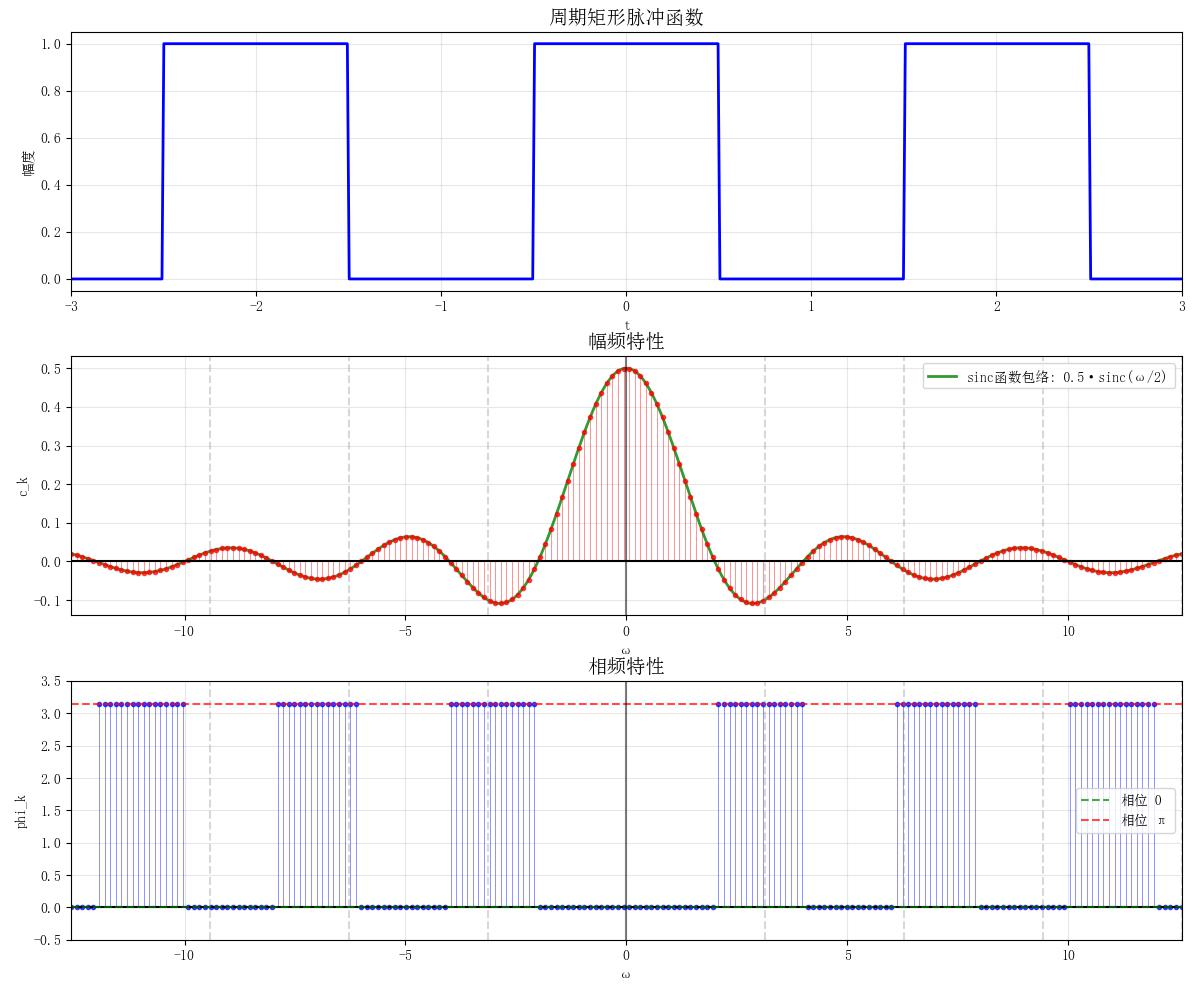
\includegraphics[width=0.6\textwidth]{Figure_2}\label{fig:2.1}
    \caption{周期矩形脉冲信号及其频谱}
\end{figure}

如图\ref{fig:2.1},可以看到,这个频谱与取样函数$Sa(\omega)$非常相似(为了体现这一点,绘制频谱时将
基波角频率大幅减小,并不是第一张图直接做傅里叶级数展开的结果),原因将在\ref{sec:Fourier}
中给出。

\textbf{带宽} (bandwidth)指最高频率与最低频率之差,表征信号频率的集中程度。对
于实信号,有时仅考虑正频率,带宽减半。周期矩形脉冲信号的频谱是无限的,但能量基
本集中在最靠近y轴的两个零点之间,此时可以将带宽定义为\textbf{第一过零点带宽}
$B=\frac{2\pi}{\tau}$(仅考虑正频率)。

\section{傅里叶变换初步}\label{sec:Fourier}
在构建傅里叶级数时,使用频率和角频率只涉及书写问题,因为傅里叶级数不会涉及尺度
变换、逆变换和卷积,但在傅里叶变换的理论中,这将导致许多公式在形式上有一些差别。
这时,将同时给出两种傅里叶变换的公式,左侧为频率版本,用蓝色标注,右侧为角频率
版本,用红色标注。对于频率的符号,物理上一般使用f或$\nu $,而一些傅里叶分析的
书上则使用s或$\xi$,但鉴于f常常用来表示信号或函数,s用于表示复频率,我们将使用$\xi$
作为频率的符号。

定义傅里叶变换的一种动机是从傅里叶级数出发。要从傅里叶级数研究的周期现象转向傅
里叶变换研究的非周期现象,自然能够想到在傅里叶级数相关的理论中,令T趋于无穷;
另一方面,复指数函数比三角函数更适合作为描述振荡(周期)行为的基本函数,因为在三角函数形式的傅
里叶级数中,无法有效地区分正频率、负频率,也难以确定应该用正弦还是余弦。

我们做一个简单的尝试,令$f\in L^2(\mathbb{R})$(关于$L^2$空间的讨论,见\ref{sec:Linear_Space}),$T\to \infty$
,则\[c_n=\frac{1}{T}\int_{T}f(t)e^{-ik\omega t}\,dt=\frac{1}{T}\int_{T}f(t)e^{-2\pi ik\xi t}\,dt\to 0\]
这样做变换将丢失f的所有信息,不是我们希望看到的,但很明显,只要给以上公式乘上T,并认为$k\omega$
或$k\xi$是自变量,问题就迎刃而解,得到一个很有意思的积分变换,它正是\textbf{傅里叶变换} (Fourier Tansform,FT):
\lr{
    \mathcal{F} f(\xi)=\int_{-\infty}^{\infty}f(t)e^{-2\pi i\xi t}\,dt
}{
    \mathcal{F} f(\omega)=\int_{-\infty}^{\infty}f(t)e^{-i\omega t}\,dt
}

有时也用$\hat{f}$或F表示f的傅里叶变换,记作
\[f\overset{\mathcal{F} }{\longleftrightarrow}F\]
并称之为\textbf{傅里叶变换对}。傅里叶变换没有最好的符号,在不引起歧义时采用最
简洁和便于理解的即可。其实,在傅里叶变换的理论中,要求$f\in L^1(\mathbb{R})$
而不是$L^2(\mathbb{R})$,$\mathbb{R}$是无穷区间,$L^1(\mathbb{R})$与
$L^2(\mathbb{R})$之间不存在包含关系。可以验证,$f\in L^1(\mathbb{R})$时,它的
傅里叶变换存在并且是连续的:\begin{align*}
    |\mathcal{F} f(\xi)|                      & =\left|\int_{-\infty}^{\infty}f(t)e^{-2\pi i\xi t}\,dt\right|                       \\
                                              & \leq\int_{-\infty}^{\infty}|f(t)||e^{-2\pi i\xi t}|\,dt<\infty                      \\
    |\mathcal{F} f(\xi+h)-\mathcal{F} f(\xi)| & =\left|\int_{-\infty}^{\infty}f(t)(e^{-2\pi i(\xi+h)t}-e^{-2\pi i\xi t})\,dt\right| \\
                                              & \leq\int_{-\infty}^{\infty}|f(t)||e^{-2\pi iht}-1|\,dt\to 0(h\to 0)
\end{align*}
另外,$\mathcal{F} f(x)\to 0(x\to\infty)$,这个结果称为\textbf{黎曼-勒贝格引理} (Riemann-Lebesgue Lemma)。

下面解释“乘T,认为$k\omega$或$k\xi$为自变量”的本质。我们来看上一节\ref{sec:Fourier_Series}
末尾的例子,为了体现双边频谱与取样函数的相似性,我们取了一个较为特殊的周期矩形
脉冲信号,它的基波角频率应为图\ref{fig:2.1}中两相邻竖直线间的间隔,即\textbf{谱线间隔},可见其频率极
小、周期极大,与我们研究非周期现象所用到的极限情况$T\to\infty$是一致的,换言之,
令$T\to\infty$自动地使“傅里叶系数”在频谱中的间隔变小,\textbf{周期信号趋向非
    周期信号的过程自动地使离散频谱趋向连续频谱}。这样,乘T就不难理解了,它的作
用是“除以$\frac{1}{T}$”,$\frac{1}{T}$是所在频率成分处小矩形的宽(类似于黎曼
积分),换言之,以频率$\xi$为横坐标,\textbf{谱系数}$c_n$是$\frac{n}{T}=n\xi$处的小矩形面积,
$Tc_n$是f中对应频率成分的含量,可以理解为单位频段内的谱系数,即频谱密度;以角频
率$\omega$为横坐标,$c_n$是$\frac{2\pi n}{T}=n\omega$处的小矩形面积,
$Tc_n$是f中对应角频率成分的含量。因此,$F(\xi)$或$F(\omega)$也称为频谱密度函
数。

实际上,从这个角度出发,可以立即得到\textbf{傅里叶逆变换} (Inverse Fourier Tansform,IFT)
的公式,因为我们已经将f展开为傅里叶级数,这对应着由f的傅里叶变换$\mathcal{F} f$
还原出f。我们知道
\lr{
f(t)&=\sum_{n=-\infty}^{\infty}c_n e^{2\pi i\xi t}\\
&=\frac{1}{T}\sum_{n=-\infty}^{\infty}(\int_{T}f(t)e^{-2\pi i\xi t}\,dt)e^{2\pi i\xi t}
}{
f(t)&=\sum_{n=-\infty}^{\infty}c_n e^{i\omega t}\\
&=\frac{1}{T}\sum_{n=-\infty}^{\infty}(\int_{T}f(t)e^{-i\omega t}\,dt)e^{i\omega t}
}
根据前文所述的对应关系,做以下替换(注意$T\to\infty$):
\lr{
    \frac{1}{T}\rightarrow d\xi,\int_{T}f(t)e^{-2\pi i\xi t}\,dt\rightarrow \mathcal{F} f(\xi)\\
    f(t)=\mathcal{F} ^{-1}\mathcal{F} (t)=\int_{-\infty}^{\infty}\mathcal{F} f(\xi)e^{2\pi i\xi t}\,d\xi
}{
    \frac{2\pi}{T}\rightarrow d\omega,\int_{T}f(t)e^{i\omega t}\,dt\rightarrow \mathcal{F} f(\omega)\\
    f(t)=\mathcal{F} ^{-1}\mathcal{F} (t)=\frac{1}{2\pi}\int_{-\infty}^{\infty}\mathcal{F} f(\omega)e^{i\omega t}\,d\omega
}
这里$\mathcal{F} ^{-1}$表示取IFT,和$\mathcal{F} $一样,是一种从函数空间到函
数空间的映射(具体是什么函数空间,我们将在\ref{sec:distributions}中讨论,目前
可以理解为$L^1(\mathbb{R})$),$\mathcal{F} $
是从时域函数到频域(角频域)函数的映射,$\mathcal{F} ^{-1}$是从频域(角频域)
到时域函数的映射。因此,严格来说我们总应该写上自变量,但在不引起歧义的情况
下允许略去,例如我们同时承认$F(\xi)=\mathcal{F} [f(t)](\xi)$和
$F(\xi)=\mathcal{F} [f(t)]$的写法。

我们从傅里叶级数类比得到了傅里叶变换及其逆变换的定义,但还没有严格证
明逆变换将给出原有的时域函数,即著名的\textbf{傅里叶反演公式} (the Fourier Inversion Thoerem),
证明将在\ref{sec:approach}给出,而不会导致循环论证。现在先介绍一些傅里叶变
换的性质,在实际计算傅里叶变换时,常常不会带入定义计算,而是通过这样的运算性质
来计算。
{\nolinebreak[4]
\begin{itemize}
    \item \textbf{对偶性}:记反转信号 (the reversed siganl)为$f^-(t)=f(-t)$,则
          \lr{(\mathcal{F}f)^-=\mathcal{F} (f^-)=\mathcal{F} ^{-1}f\\
              \mathcal{F} \mathcal{F} f=f^-\\
              f\text{是实信号}\Rightarrow \mathcal{F} f^-=\overline{\mathcal{F} f}
          }{(\mathcal{F}f)^-=\mathcal{F} (f^-)=2\pi\mathcal{F} ^{-1}f\\
              \mathcal{F} \mathcal{F} f=2\pi f^-\\
              f\text{是实信号}\Rightarrow \mathcal{F} f^-=\overline{\mathcal{F} f}}
          时域反转,频域也反转,因此我们可以不区分$(\mathcal{F}f)^-=\mathcal{F} (f^-)$,将它们全部写作$\mathcal{F} f^-$.\\
          不涉及收敛性的问题时,的确可以做多次傅里叶变换,只是此时不再具有明显的物理意义,因而也不纠结所选用的符号。
    \item \textbf{对称性}:$\mathcal{F} f$与f奇偶性相同;f是实函数时,如果f还是偶函数,则$\mathcal{F} f$也是实函数,
          如果f还是奇函数,则$\mathcal{F} $是纯虚函数
    \item \textbf{线性性}:$\forall f,g\in L^1(\mathbb{R}),\mathcal{F} (af+bg)=a\mathcal{F} f+b\mathcal{F} g$,即$\mathcal{F} $是线性算子
    \item \textbf{平移定理}:\lr{
          &\mathcal{F} [f(t-b)](\xi)=e^{-2\pi i \xi b}\mathcal{F} f(\xi)\\
          &\mathcal{F} [f(t)e^{2\pi i \xi t}]=\mathcal{F} f(\xi-b)
          }{
          &\mathcal{F} [f(t-b)](\omega)=e^{-i\omega t}\mathcal{F} f(\omega)\\
          &\mathcal{F} [f(t)e^{ibt}](\omega)=\mathcal{F} f(\omega-b)
          }
          可见信号时移$|\mathcal{F} f|$,而仅改变$\mathcal{F} f$的相位。
    \item \textbf{伸缩定理}:\lr{
              &\mathcal{F} [f(at)](\xi)=\frac{1}{|a|}\mathcal{F} f(\frac{\xi}{a})\\
            &\mathcal{F} f(a\xi)=\frac{1}{|a|}\mathcal{F} [f(\frac{t}{a})]
          }{
              &\mathcal{F} [f(at)](\omega)=\frac{1}{|a|}\mathcal{F} f(\frac{\omega}{a})\\
              &\mathcal{F} f(a\xi)=\frac{1}{|a|}\mathcal{F} [f(\frac{t}{a})]
          }
          信号反转可看作a=-1的特例。可以认为两种频率下的傅里叶变换是通过伸缩得到的,即
          \[2\pi\xi=\omega,\textcolor{blue}{\mathcal{F}}(2\pi\xi)=\textcolor{red}{\mathcal{F}}(\omega)\]
          a>1,时域收缩,频域舒张、变矮;0<a<1,时域舒张,频域收缩、变高;a<0,时域和频域都额外做一次反转。
    \item \textbf{微分性质}:\lr{
              &\mathcal{F} (f')(\xi)=2\pi i\xi\mathcal{F} f(\xi)\\
              &\mathcal{F}(2\pi itf)(\xi)=-(\mathcal{F} f)'(\xi)\\
              &\text{即}\mathcal{F}(tf)(\xi)=\frac{i}{2\pi}(\mathcal{F} f)'(\xi)
          }{
              &\mathcal{F} (f')(\omega)=i\omega\mathcal{F} f(\omega)\\
              &\mathcal{F} [itf(t)](\omega)=-(\mathcal{F} f)'(\omega)\\
              &\text{即}\mathcal{F}(tf)(\omega)=i(\mathcal{F} f)'(\omega)
          }
          最后一步使用了线性性;容易将此性质推广至任意阶导数。
\end{itemize}
\textbf{Proof:}\\
1.对偶性
\lr{
    (\mathcal{F} f)^-(\xi)&=\int_{-\infty}^{\infty}f(t)e^{2\pi i \xi t}\,dt\\
    \mathcal{F} (f^-)(\xi)&=\int_{-\infty}^{\infty}f(-t)e^{-2\pi i \xi t}\,dt\\
    &=\int_{-\infty}^{\infty}f(t)e^{2\pi i \xi t}\,dt\\
    \mathcal{F} ^{-1}f(x)&=\int_{-\infty}^{\infty}f(t)e^{2\pi ixt}\,dt
}{
    (\mathcal{F} f)^-(\omega)&=\int_{-\infty}^{\infty}f(t)e^{i \omega t}\,dt\\
    \mathcal{F} (f^-)(\omega)&=\int_{-\infty}^{\infty}f(-t)e^{-i \omega t}\,dt\\
    &=\int_{-\infty}^{\infty}f(t)e^{i \omega t}\,dt\\
    \mathcal{F} ^{-1}f(x)&=\frac{1}{2\pi}\int_{-\infty}^{\infty}f(t)e^{i\omega t}\,dt
}
因此\lr{(\mathcal{F}f)^-=\mathcal{F} (f^-)=\mathcal{F} ^{-1}f}{(\mathcal{F}f)^-=\mathcal{F} (f^-)=2\pi\mathcal{F} ^{-1}f}
同时取傅里叶变换,即得
\lr{
    &\mathcal{F} \mathcal{F} f=f^-\\
    &\text{f是实信号时,}f=\overline{f},\\
    &\mathcal{F} f^-(\xi)=\int_{-\infty}^{\infty}f(t)e^{2\pi i \xi t}\,dt\\
    &\ =\overline{\int_{-\infty}^{\infty}f(t)e^{-2\pi i \xi t}\,dt}=\overline{\mathcal{F} f(\xi)}
}{
    &\mathcal{F} \mathcal{F} f=2\pi f^-\\
    &\text{f是实信号时,}f=\overline{f},\\
    &\mathcal{F} f^-(\omega)=\int_{-\infty}^{\infty}f(t)e^{i \omega t}\,dt\\
    &\ =\overline{\int_{-\infty}^{\infty}f(t)e^{-i \omega t}\,dt}=\overline{\mathcal{F} f(\omega)}
}}
\noindent 2.对称性\\
根据对偶性立即得到。\\
3.线性性\\
得自积分的线性性。\\
4.平移定理
\lr{
\mathcal{F} [f(t-b)](\xi)&=\int_{-\infty}^{\infty}f(t-b)e^{-2\pi i \xi t}\,dt\\
&=\int_{-\infty}^{\infty}f(t)e^{-2\pi i \xi (t+b)}\,dt\\
&=e^{-2\pi i \xi b}\int_{-\infty}^{\infty}f(t)e^{-2\pi i \xi t}\,dt\\
&=e^{-2\pi i \xi b}\mathcal{F} f(\xi)\\
\mathcal{F} f(\xi-b)&=\int_{-\infty}^{\infty}f(t)e^{-2\pi i(\xi-b)t}\,dt\\
&=\int_{-\infty}^{\infty}\left(f(t)e^{2\pi ibt}\right)e^{-2\pi i\xi t}\,dt\\
&=\mathcal{F} [f(t)e^{2\pi ibt}](\xi)
}{
\mathcal{F} [f(t-b)](\omega)&=\int_{-\infty}^{\infty}f(t-b)e^{-i \omega t}\,dt\\
&=\int_{-\infty}^{\infty}f(t)e^{-i \omega (t+b)}\,dt\\
&=e^{-i \omega b}\int_{-\infty}^{\infty}f(t)e^{-i \omega t}\,dt\\
&=e^{-i \omega b}\mathcal{F} f(\omega)\\
\mathcal{F} f(\omega-b)&=\int_{-\infty}^{\infty}f(t)e^{-i(\omega-b)t}\,dt\\
&=\int_{-\infty}^{\infty}\left(f(t)e^{ibt}\right)e^{-i\omega t}\,dt\\
&=\mathcal{F} [f(t)e^{ibt}](\xi)
}
\noindent 5.伸缩定理\lr{
    \mathcal{F} [f(at)](\xi)&=\int_{-\infty}^{\infty}f(at)e^{2\pi i \xi t}\,dt\\
    &=\frac{1}{|a|}\int_{-\infty}^{\infty}f(t)e^{\frac{2\pi i \xi t}{a}}\,dt\text{(变量代换)}\\
    &=\frac{1}{|a|}\mathcal{F} f(\frac{\xi}{a})
}{
    \mathcal{F} [f(at)](\omega)&=\int_{-\infty}^{\infty}f(at)e^{i \omega t}\,dt\\
    &=\frac{1}{|a|}\int_{-\infty}^{\infty}f(t)e^{\frac{i \omega t}{a}}\,dt\text{(变量代换)}\\
    &=\frac{1}{|a|}\mathcal{F} f(\frac{\omega}{a})
}
注意变量代换时,如果a<0,积分上下限也会改变,这正是绝对值的来源,对此有疑惑的读者
可以自行分情况验算。对于频域的伸缩定理,仅仅是时域伸缩定理的直接推论。\\
6.微分性质
\lr    {
\mathcal{F} (f')(\xi)&=\int_{-\infty}^{\infty}f'(t)e^{-2\pi i\xi t}\,dt\\
&=\int_{-\infty}^{\infty}e^{-2\pi i\xi t}\,df(t)\\
&=\evalat{e^{-2\pi i\xi t}f(t)}{-\infty}{\infty}+2\pi i\xi\int_{-\infty}^{\infty}f(t)e^{-2\pi i\xi t}\,dt\\
&=2\pi i\xi\mathcal{F} f(\xi)\\
(\mathcal{F} f)'(\xi)&=\frac{d}{d\xi}\int_{-\infty}^{\infty}f(t)e^{-2\pi i\xi t}\,dt\\
&=\int_{-\infty}^{\infty}f(t)\frac{\partial e^{-2\pi i\xi t}}{\partial \xi}\,dt\\
&=-\int_{-\infty}^{\infty}2\pi itf(t)e^{-2\pi i\xi t}\,dt\\
&=-\mathcal{F} (2\pi itf)(\xi)
}{
\mathcal{F} (f')(\omega)&=\int_{-\infty}^{\infty}f'(t)e^{-i\omega t}\,dt\\
&=\int_{-\infty}^{\infty}e^{-i\omega t}\,df(t)\\
&=\evalat{e^{-i\omega t}f(t)}{-\infty}{\infty}+i\omega\int_{-\infty}^{\infty}f(t)e^{-i\omega t}\,dt\\
&=i\omega\mathcal{F} f(\omega)\\
(\mathcal{F} f)'(\omega)&=\frac{d}{d\omega}\int_{-\infty}^{\infty}f(t)e^{-i\omega t}\,dt\\
&=\int_{-\infty}^{\infty}f(t)\frac{\partial e^{-i\omega t}}{\partial \omega}\,dt\\
&=-\int_{-\infty}^{\infty}itf(t)e^{-i\omega t}\,dt\\
&=-\mathcal{F} (itf)(\omega)
}
$\evalat{e^{-2\pi i\xi t}f(t)}{-\infty}{\infty},\evalat{e^{-i\omega t}f(t)}{-\infty}{\infty}=0$
是因为$f\in L^1(\mathbb{R})$要求反常积分$\int_{\mathbb{R}}|f(t)|\,dt<\infty$
,其必要条件为$f(t)\to 0,t\to\infty$,而复指数函数部分模值恒为1。对于后一等式
中将求导与积分交换的操作,实际上是\textbf{莱布尼兹积分法则},也即含参变量积分
的求导,通常需要条件(以角频率形式为例)\begin{circlist}
    \item $\int_{-\infty}^{\infty}f(t)e^{-i\omega t}\,dt$对每个$\omega$可积
    \item $\frac{\partial f(t)e^{-i\omega t}}{\partial \omega}=-itf(t)e^{-i\omega t}$存在
    \item 存在可积函数$g(t)$使得$|-itf(t)e^{-i\omega t}|\leq g(t)$
\end{circlist}
\ding{174}成立是因为定理假设$f(t),tf(t)$能够进行傅里叶变换,从而
$f(t),tf(t)\in L^1(\mathbb(R)),g(t)=tf(t)$.
工程上一般不涉及这些,仅作形式计算。也可以由第一个微分性质取傅里叶逆变换,再令
$f'=\mathcal{F} g$。

下面介绍一些常用信号的傅里叶变换,并使用傅里叶反演公式和对偶性得到一些难以直接
计算的常用傅里叶变换。

\noindent 例3.1.在\ref{sec:Fourier_Series}中讨论了矩形函数$f(t)=E\cdot\Pi_T(t)$的傅里
叶变换,现在可以验证它的频谱与取样函数相似:
\lr{
\mathcal{F} f(\xi)&=\int_{-\infty}^{\infty}f(t)e^{-2\pi i\xi t}\,dt\\
&=E\int_{-\infty}^{\infty}\Pi_T(t)e^{-2\pi i\xi t}\,dt\\
&=E\int_{-\frac{T}{2}}^{\frac{T}{2}}e^{-2\pi i\xi t}\,dt\\
&=-\frac{E}{2\pi i\xi}\evalat{e^{-2\pi i\xi t}}{-\frac{T}{2}}{\frac{T}{2}}\\
&=\frac{e^{\pi i\xi T}-e^{-\pi i\xi T}}{2i}\frac{E}{\pi\xi}\\
&=\frac{E}{\pi\xi}\sin(\pi T\xi)=ETsinc(T\xi)
}{
\mathcal{F} f(\omega)&=\int_{-\infty}^{\infty}f(t)e^{-i\omega t}\,dt\\
&=E\int_{-\infty}^{\infty}\Pi_T(t)e^{-i\omega t}\,dt\\
&=E\int_{-\frac{T}{2}}^{\frac{T}{2}}e^{-i\omega t}\,dt\\
&=-\frac{E}{i\omega}\evalat{e^{-i\omega t}}{-\frac{T}{2}}{\frac{T}{2}}\\
&=\frac{e^{\frac{i\omega T}{2}}-e^{-\frac{i\omega T}{2}}}{2i}\frac{2E}{\pi\omega}\\
&=\frac{2E}{\omega}\sin(\frac{T\omega}{2})=ETSa(\frac{T\omega}{2})
}
因此\lr{
    \mathcal{F} \Pi_T(\xi)&=Tsinc(T\xi)\\
    \mathcal{F} sinc(\xi)&=\Pi(\xi)
}{
    \mathcal{F} \Pi_T(\omega)&=TSa(\frac{T\omega}{2})\\
    \mathcal{F} Sa(\frac{\omega}{2})&=\frac{1}{2}\Pi_2 (\omega)
}

\noindent 例3.2.在\ref{sec:signal}中介绍了狄拉克$\delta$函数,实际上它应该作为一个分布来理解,
见\ref{sec:distributions},不过我们可以从形式上求出它的傅里叶变换。
\lr{
\mathcal{F} \delta(\xi)&=\int_{-\infty}^{\infty}\delta(t)e^{-2\pi i\xi t}\,dt\\
&=\int_{-\infty}^{\infty}\delta(t)\,dt=1
}{
\mathcal{F} \delta(\omega)&=\int_{-\infty}^{\infty}\delta(t)e^{-i\omega t}\,dt\\
&=\int_{-\infty}^{\infty}\delta(t)\,dt=1
}
根据傅里叶变换的对偶性,我们当然希望恒为1的函数的傅里叶变换是$\delta$或$2\pi\delta$
(取决于是用频率做变换还是用角频率做变换),然而,1在无限区间上必定是不可积的,
在常规意义下它不能够做傅里叶变换。这个问题将在\ref{sec:distributions}中讨论,
那时就可以对相当大范围内的函数做傅里叶变换,还将看到周期函数的傅里叶变换与傅里
叶级数的深刻关系。现在我们暂且承认公式\lr{
    &\mathcal{F} \delta(\xi)=1\\
    &\mathcal{F} \mathds{1}=\delta(\xi)
}{
    &\mathcal{F} \delta(\omega)=1\\
    &\mathcal{F} \mathds{1}=2\pi\delta(\omega)
}
其中$\mathds{1}$表示恒为1的函数。根据傅里叶变换的平移定理,立即得到:
\lr{
\mathcal{F} [\delta_a](\xi)&=e^{-2\pi i\xi a}\\
\mathcal{F} [e^{2\pi ia t}]&=\delta_a
}{
\mathcal{F} [\delta_a](\omega)&=e^{-i\omega a}\\
\mathcal{F} [e^{ia t}]&=2\pi\delta_a
}
根据傅里叶变换的微分性质得到:\lr{
    \mathcal{F} [t^n](\xi)&=(\frac{i}{2\pi})^n \delta^{(n)}(\xi)\\
}{
    \mathcal{F} [t^n](\omega)&=(i)^n \cdot 2\pi \delta^{(n)}(\omega)\\
}
我们还希望从$u'(t)=\delta(t),sgn'(t)=2\delta(t)$
得到单位阶跃函数u(t)和符号函数sgn(t)的傅里叶变换,但在考虑$\delta$的不定积分时,必须
处理“C”,它将导致频域中出现$C\delta$或$2\pi C\delta$项。注意到$sgn(t)$是奇函数,我
们可以由此确定它和单位阶跃函数的傅里叶变换中C的值,从而得到正确的结果:
\lr{
\mathcal{F} sgn(\xi)&=\frac{1}{\pi i\xi}\\
\mathcal{F} u(\xi)&=\mathcal{F} [\frac{1}{2}(sgn(t)+1)]\\
&=\frac{1}{2}(\delta+\frac{1}{\pi i\xi})\\
}{
\mathcal{F} sgn(\omega)&=\frac{2}{i\omega}\\
\mathcal{F} u(\omega)&=\mathcal{F} [\frac{1}{2}(sgn(t)+1)]\\
&=\pi\delta+\frac{1}{i\omega}\\
}
用傅里叶反演公式,
\lr{
    \mathcal{F} [\frac{1}{t}](\xi)&=-\pi i sgn(\xi)\\
}{
    \mathcal{F} [\frac{1}{t}](\omega)&=-\pi i sgn(\omega)\\
}

\noindent 例3.3. $\Lambda$函数,它在卷积的章节中是一个很好的例子。
\[\Lambda(t)=\begin{cases}
        1-|t| & \text{if }|t|\leq 1 \\
        0     & \text{if }|t|>1
    \end{cases}\]
\begin{figure}[htbp]
    \centering
    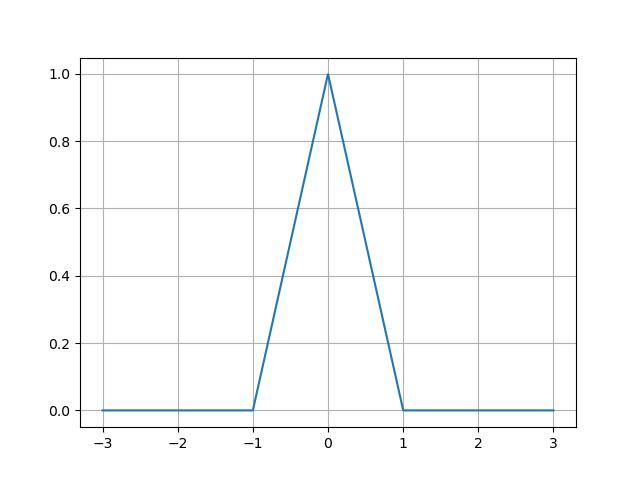
\includegraphics[width=0.4\textwidth]{lambda}
    \caption{$\Lambda$函数图像}
\end{figure}
\lr{
&\text{记$e^{2\pi i\xi t}$的原函数为}F(t)=\frac{e^{2\pi i\xi t}}{2\pi i\xi}\\
\mathcal{F} \Lambda(\xi)&=\int_{-\infty}^{\infty}\Lambda(t)e^{-2\pi i\xi t}\,dt\\
&=\int_{-1}^{0}(1+t)e^{-2\pi i\xi t}\,dt+\int_{0}^{1}(1-t)e^{-2\pi i\xi t}\,dt\\
&=F(1)-F(-1)-\frac{1}{2\pi i\xi}\left(\evalat{t e^{-2\pi i\xi t}}{-1}{0}\right. \\
&\ \left.\ -\int_{-1}^{0}e^{-2\pi i\xi t}\,dt-\evalat{t e^{-2\pi i\xi t}}{0}{1}+\int_{0}^{1}e^{-2\pi i\xi t}\,dt\right)\\
&=\frac{F(1)-2F(0)+F(-1)}{2\pi i\xi}\\
&=\frac{e^{2\pi i\xi}+e^{-2\pi i\xi}-2}{(2\pi i\xi)^2}=\frac{1}{(\pi\xi)^2}(\frac{e^{\pi\xi}-e^{-\pi\xi}}{2i})^2\\
&=sinc^2(\xi)
}{
&\text{记$e^{i\omega t}$的原函数为}F(t)=\frac{e^{i\omega t}}{i\omega}\\
\mathcal{F} \Lambda(\omega)&=\int_{-\infty}^{\infty}\Lambda(t)e^{-i\omega t}\,dt\\
&=\int_{-1}^{0}(1+t)e^{-i\omega t}\,dt+\int_{0}^{1}(1-t)e^{-i\omega t}\,dt\\
&=F(1)-F(-1)-\frac{1}{i\omega}\left(\evalat{t e^{-i\omega t}}{-1}{0}\right. \\
&\ \left.\ -\int_{-1}^{0}e^{-i\omega t}\,dt-\evalat{t e^{-i\omega t}}{0}{1}+\int_{0}^{1}e^{-i\omega t}\,dt\right)\\
&=\frac{F(1)-2F(0)+F(-1)}{i\omega}\\
&=\frac{e^{i\omega}+e^{-i\omega}-2}{(i\omega)^2}=\frac{4}{(\omega)^2}(\frac{e^{\frac{\omega}{2}}-e^{-\frac{\omega}{2}}}{2i})^2\\
&=Sa^2(\frac{\omega}{2})
}
因此\lr{
    \mathcal{F} sinc^2(\xi)&=\Lambda(t)\\
}{
    \mathcal{F} Sa^2(\frac{\omega}{2})&=\Lambda(t)
}

\noindent 例3.4. 高斯函数 $G(t)=\frac{1}{\sqrt{2\pi}\sigma}e^{-\frac{t^2}{2\sigma^2}}$,求它的傅里叶变换的方法较为特殊:
\lr{
\mathcal{F} G(\xi)&=\int_{-\infty}^{\infty}\frac{1}{\sqrt{2\pi}\sigma}e^{-\frac{t^2}{2\sigma^2}}e^{-2\pi i\xi t}\,dt\\
\frac{d}{d\xi}\mathcal{F} G(\xi)&=\int_{-\infty}^{\infty}\frac{1}{\sqrt{2\pi}\sigma}e^{-\frac{t^2}{2\sigma^2}}(-2\pi it)e^{-2\pi i\xi t}\,dt\\
&=2\pi i\sigma^2\int_{-\infty}^{\infty}e^{-2\pi i\xi t}\,d\frac{1}{\sqrt{2\pi}\sigma}e^{-\frac{t^2}{2\sigma^2}}\\
&=-4\pi^2\sigma^2\xi\int_{-\infty}^{\infty}\frac{1}{\sqrt{2\pi}\sigma}e^{-\frac{t^2}{2\sigma^2}}e^{-2\pi i\xi t}\,dt\\
&=-4\pi^2\sigma^2\xi\mathcal{F} G
}{
\mathcal{F} G(\omega)&=\int_{-\infty}^{\infty}\frac{1}{\sqrt{2\pi}\sigma}e^{-\frac{t^2}{2\sigma^2}}e^{-i\omega t}\,dt\\
\frac{d}{d\xi}\mathcal{F} G(\xi)&=\int_{-\infty}^{\infty}\frac{1}{\sqrt{2\pi}\sigma}e^{-\frac{t^2}{2\sigma^2}}(-it)e^{-i\omega t}\,dt\\
&=i\sigma^2\int_{-\infty}^{\infty}e^{-i\omega t}\,d\frac{1}{\sqrt{2\pi}\sigma}e^{-\frac{t^2}{2\sigma^2}}\\
&=-\sigma^2\omega\int_{-\infty}^{\infty}\frac{1}{\sqrt{2\pi}\sigma}e^{-\frac{t^2}{2\sigma^2}}e^{-i\omega t}\,dt\\
&=-\sigma^2\omega\mathcal{F} G
}
这是一个可分离变量的微分方程,
\lr{
\mathcal{F} G(\xi)&=\mathcal{F} G(0)e^{-2\pi^2\sigma^2\xi^2}\\
\mathcal{F} G(0)&=\int_{-\infty}^{\infty}\frac{1}{\sqrt{2\pi}\sigma}e^{-\frac{t^2}{2\sigma^2}}\,dt=1\\
\mathcal{F} G(\xi)&=e^{-2\pi^2\sigma^2\xi^2}
}{
\mathcal{F} G(\omega)&=\mathcal{F} G(0)e^{-\frac{\sigma^2\omega^2}{2}}\\
\mathcal{F} G(0)&=\int_{-\infty}^{\infty}\frac{1}{\sqrt{2\pi}\sigma}e^{-\frac{t^2}{2\sigma^2}}\,dt=1\\
\mathcal{F} G(\xi)&=e^{-\frac{\sigma^2\omega^2}{2}}
}
\begin{figure}[htbp]
    \centering
    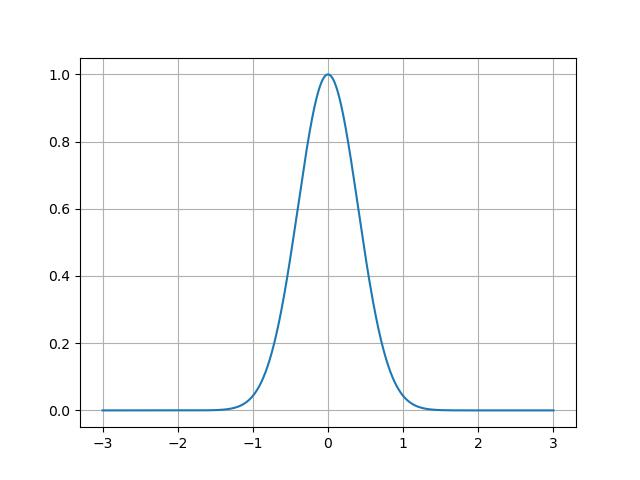
\includegraphics[width=0.4\textwidth]{Gauss}
    \caption{高斯函数图像}
\end{figure}

\noindent 例3.5. 单边指数函数$f(t)=\begin{cases}
        e^{-at}, & \text{if }t\geq 0 \\
        0,       & \text{if }t<0
    \end{cases}$和双边指数函数$g(t)=\begin{cases}
        e^{-at}, & \text{if }t\geq 0 \\
        e^{at},  & \text{if }t<0
    \end{cases}$\\
\lr{
\mathcal{F} f(\xi)&=\int_{-\infty}^{\infty}f(t)e^{-2\pi i\xi t}\,dt\\
&=\int_{0}^{\infty}e^{-at}e^{-2\pi i\xi t}\,dt\\
&=-\frac{1}{a+2\pi i\xi}\left.e^{-(a+2\pi i\xi)t}\right|_{0}^{\infty}\\
&=\frac{1}{a+2\pi i\xi}
}{
\mathcal{F} f(\omega)&=\int_{-\infty}^{\infty}f(t)e^{-i\omega t}\,dt\\
&=\int_{0}^{\infty}e^{-at}e^{-i\omega t}\,dt\\
&=-\frac{1}{a+i\omega}\left.e^{-(a+i\omega)t}\right|_{0}^{\infty}\\
&=\frac{1}{a+i\omega}
}
运用对偶性,立即得到
\lr{
\mathcal{F} g(\xi)&=\mathcal{F} f(\xi)+\overline{\mathcal{F} f(\xi)}\\
&=2Re{\mathcal{F} f(\xi)}=\frac{2a}{a^2 + 4\pi^2 \xi^2}
}{
\mathcal{F} g(\omega)&=\mathcal{F} f(\omega)+\overline{\mathcal{F} f(\omega)}\\
&=2Re{\mathcal{F} f(\omega)}=\frac{2a}{a^2 +\omega^2}
}

最后,我们给出\textbf{帕塞瓦尔恒等式}(Parceval's identity):\lr{
    \int_{-\infty}^{\infty}|f(t)|^2\,dt=\int_{-\infty}^{\infty}|\mathcal{F} f(\xi)|^2\,d\xi
}{
    \int_{-\infty}^{\infty}|f(t)|^2\,dt=\frac{1}{2\pi}\int_{-\infty}^{\infty}|\mathcal{F} f(\omega)|^2\,d\omega
}
\textbf{Proof:}设$f,g\in L^1(\mathbb{R})$,\lr{
    &\quad\int_{-\infty}^{\infty}\mathcal{F} f(\xi)\overline{\mathcal{F} g(\xi)}\,d\xi\\
    &=\int_{-\infty}^{\infty}\mathcal{F} f(\xi)\mathcal{F}^{-1} \overline{g}(\xi)\,d\xi\\
    &=\int_{-\infty}^{\infty}\left(\int_{-\infty}^{\infty}f(x)e^{-2\pi i\xi x}\,dx\right)\mathcal{F}^{-1} \overline{g}(\xi)\,d\xi\\
    &=\int_{-\infty}^{\infty}f(x)\,dx\int_{-\infty}^{\infty}\mathcal{F}^{-1} \overline{g}(\xi)e^{-2\pi i\xi x}\,d\xi\\
    &=\int_{-\infty}^{\infty}f(x)\mathcal{F} \mathcal{F} ^{-1}\overline{g}(x)\,dx\\
    &=\int_{-\infty}^{\infty}f(x)\overline{g(x)}\,dx
}{
    &\quad\int_{-\infty}^{\infty}\mathcal{F} f(\omega)\overline{\mathcal{F} g(\omega)}\,d\omega\\
    &=2\pi\int_{-\infty}^{\infty}\mathcal{F} f(\omega)\mathcal{F}^{-1} \overline{g}(\omega)\,d\omega\\
    &=2\pi\int_{-\infty}^{\infty}\left(\int_{-\infty}^{\infty}f(x)e^{-i\omega x}\,dx\right)\mathcal{F}^{-1} \overline{g}(\omega)\,d\omega\\
    &=2\pi\int_{-\infty}^{\infty}f(x)\,dx\int_{-\infty}^{\infty}\mathcal{F}^{-1} \overline{g}(\omega)e^{-i\omega x}\,d\omega\\
    &=2\pi\int_{-\infty}^{\infty}f(x)\mathcal{F} \mathcal{F} ^{-1}\overline{g}(x)\,dx\\
    &=2\pi\int_{-\infty}^{\infty}f(x)\overline{g(x)}\,dx
}
取$g=f$即证。注意我们并不要求$g$是实信号,$\overline{\mathcal{F} g}\neq\mathcal{F} ^{-1}g$.

\section{卷积}\label{sec:convolution}

信号处理讨论的一个基本问题是\textbf{滤波},即希望把一个信号输入滤波系统后,输
出的信号的一些频率成分被剔除或大幅减少,以低通滤波器为例,从数学上讲,就是把信
号的频域形式乘以一个矩形函数或一个在给定的频率值之外快速下降到接近于0的函数,
这就引出了一个问题:在频域乘一个函数,在时域上的表现是什么?我们知道,一般而言
没有$\mathcal{F} (fg)=\mathcal{F} f\mathcal{F} g$。一个自然的想法是,看能
否定义一种运算,使得在频域乘一个函数,相当于在时域与这个函数的时域形式做该种运
算。实际上,这种运算是存在的,它正是\textbf{卷积}(convolution)

下面就来找出这个运算。设$f\overset{\mathcal{F} }{\longleftrightarrow}F,g\overset{\mathcal{F} }{\longleftrightarrow}G$,
\lr{
    F(\xi)G(\xi)=&\int_{-\infty}^{\infty}f(x)e^{-2\pi i\xi x}\,dx\int_{-\infty}^{\infty}g(y)e^{-2\pi i\xi y}\,dy\\
    &=\iint\limits_{\mathbb{R}^2}f(x)g(y)e^{-2\pi i\xi(x+y)}\,dx\,dy
}{
    F(\omega)G(\omega)=&\int_{-\infty}^{\infty}f(x)e^{-i\omega x}\,dx\int_{-\infty}^{\infty}g(y)e^{-i\omega y}\,dy\\
    &=\iint\limits_{\mathbb{R}^2}f(x)g(y)e^{-i\omega(x+y)}\,dx\,dy
}
令$z=x+y$,则积分区域仍为$\mathbb{R}^2$,
\[dxdz=\left|\frac{\partial(x,z)}{\partial(x,y)}\right|dxdy=\left|\begin{vmatrix}
        1 & 0 \\
        1 & 1
    \end{vmatrix}\right| dxdy=dxdy\]
\lr{
F(\xi)G(\xi)=&\iint\limits_{\mathbb{R}^2}f(x)g(z-x)e^{-2\pi i\xi z}\,dx\,dz\\
&=\int_{-\infty}^{\infty}e^{-2\pi i\xi z}\,dz\int_{-\infty}^{\infty}f(x)g(z-x)dx\\
&=\mathcal{F} [\int_{-\infty}^{\infty}f(x)g(z-x)dx](\xi)
}{
F(\omega)G(\omega)=&\iint\limits_{\mathbb{R}^2}f(x)g(z-x)e^{-i\omega z}\,dx\,dz\\
&=\int_{-\infty}^{\infty}e^{-i\omega z}\,dz\int_{-\infty}^{\infty}f(x)g(z-x)dx\\
&=\mathcal{F} [\int_{-\infty}^{\infty}f(x)g(z-x)dx](\omega)
}

因此我们定义函数f,g的\textbf{卷积}为
\begin{equation}
    (f*g)(x)=\int_{-\infty}^{\infty}f(y)g(x-y)\,dy
\end{equation}
并且有$\mathcal{F} (f*g)=\mathcal{F} f\mathcal{F} g$.以上是时域卷积的性质,由
傅里叶反演公式,不难想到频域卷积也有类似的性质。令$f=\mathcal{F} \mathfrak{f},g=\mathcal{F} \mathfrak{g}$
,对以上公式两边同时取傅里叶逆变换:
\lr{
f*g&=\mathcal{F} ^{-1}(\mathcal{F} f\mathcal{F} g)\\
\Leftrightarrow\mathcal{F} \mathfrak{f}*\mathcal{F} \mathfrak{g}&=\mathcal{F} ^{-1}[\mathcal{F}\mathcal{F} \mathfrak{f}\mathcal{F} \mathcal{F} \mathfrak{g}]\\
&=\mathcal{F} ^{-1}(\mathfrak{f}^- \mathfrak{g}^- )\\
&=\mathcal{F} (\mathfrak{fg})\\
\Leftrightarrow\mathcal{F} (fg)(\xi)&=\mathcal{F} f*\mathcal{F} g(\xi)
}{
f*g&=\mathcal{F} ^{-1}(\mathcal{F} f\mathcal{F} g)\\
\Leftrightarrow\mathcal{F} \mathfrak{f}*\mathcal{F} \mathfrak{g}&=\mathcal{F} ^{-1}[\mathcal{F}\mathcal{F} \mathfrak{f} \mathcal{F} \mathcal{F} \mathfrak{g}]\\
&=\mathcal{F} ^{-1}(4\pi^2 \mathfrak{f}^- \mathfrak{g}^- )\\
&= 2\pi\mathcal{F} (\mathfrak{fg})\\
\Leftrightarrow\mathcal{F} (fg)(\omega )&=\frac{1}{2\pi}\mathcal{F} f*\mathcal{F} g(\omega)
}
综上得到\textbf{卷积定理}(the convoluton thoerem):
\lr{
    \mathcal{F} (f*g)(\xi)=\mathcal{F} f(\xi)\mathcal{F} g(\xi)\\
    \mathcal{F} (fg)(\xi)=(\mathcal{F} f*\mathcal{F} g)(\xi)
}{
    \mathcal{F} (f*g)(\omega)=\mathcal{F} f(\omega)\mathcal{F} g(\omega)\\
    \mathcal{F} (fg)(\omega)=\frac{1}{2\pi}(\mathcal{F} f*\mathcal{F} g)(\omega)
}

上一节中我们曾花费大量的篇幅寻找$\Lambda$的傅里叶变换,现在可以用卷积定理得到
它,因为$\Lambda=\Pi_{1/2}*\Pi_{1/2}$(读者可以自行用代数方法验证)。

在不引起歧义时,我们也承认$f(t)*g(t)$和$f(t)*e^{t+1}$这样的写法。需要注意,$f(2t)*g(t)$
对应着两种理解:$\int_{-\infty}^{\infty}f(2t-x)g(x)\,dx$和$\int_{-\infty}^{\infty}f(2(t-x))g(x)\,dx$
,第二种才是对的,因为我们认为$f(2t)$作为一个新的函数$F(t)=f(2t)$与$g(t)$进行卷积。

作为一种新的函数空间上的运算,我们自然要讨论它是否满足线性性、结合律、
交换律。事实上,它们都是成立的:
\begin{align}
    f*(ag_1+bg_2) & =af*g_1+bf*g_2 \\
    (f*g)*h       & =f*(g*h)       \\
    f*g           & =g*f
\end{align}
线性性得自积分的线性性,交换律通过变量替换即可证明,下面仅证明结合律。\\
\textbf{Proof:}
\begin{align*}
    (f*g)*h(x) & =\int_{-\infty}^{\infty}(f*g)(x-y)h(y)\,dy=\int_{-\infty}^{\infty}h(y)\,dy\int_{-\infty}^{\infty}f(z)g(x-y-z)\,dz \\
               & =\int_{-\infty}^{\infty}\int_{-\infty}^{\infty}f(z)g(x-y-z)h(y)\,dy\,dz=\int_{-\infty}^{\infty}f(z)(g*h)(x-z)\,dz
\end{align*}
也可以通过取傅里叶变换的方式证明它们,但这样会缩减证明有效的范围,因为
卷积存在只要求积分$(f*g)(x)=\int_{-\infty}^{\infty}f(y)g(x-y)\,dy$
存在(它有许多种充分条件,不再一一讨论),而取傅里叶变换则要求$f,g,f*g$
的傅里叶变换存在。

接着讨论卷积是否具有“幺元”,即与任一函数卷积,总得到它本身。
\lr{
    &\mathcal{F} (f*\delta)(\xi)=\mathcal{F} f(\xi)\mathcal{F} \delta(\xi)=\mathcal{F} f(\xi)\\
    &f(t)=(f*\delta)(t)=\int_{-\infty}^{\infty}f(x)\delta(t-x)\,dx
}{
    &\mathcal{F} (f*\delta)(\omega)=\mathcal{F} f(\omega)\mathcal{F} \delta(\omega)=\mathcal{F} f(\omega)\\
    &f(t)=(f*\delta)(t)=\int_{-\infty}^{\infty}f(x)\delta(t-x)\,dx
}
因此$\delta$是“卷积幺元”,傅里叶变换构成$\langle L^1(\mathbb{R}),+,\cdot\rangle$
与$\langle \mathcal{F} (L^1(\mathbb{R})),+,*\rangle$之间的环同态。

一些简单的卷积可以通过画图法进行计算。将一个函数翻转、平移,再与另一函数相乘、
积分,就得到了它们的卷积,下面用$\Lambda=\Pi_{1/2}*\Pi_{1/2}$的例子加以说明。
$\Pi_{1/2}$是偶函数,$\Pi_{1/2}(-t)=\Pi_{1/2}(t)$.计算
$(\Pi_{1/2}*\Pi_{1/2})(x)=\int_{-\infty}^{\infty}\Pi_{1/2}(y)\Pi_{1/2}(x-y)\,dy$
时,如果$|x|>1$,则将$\Pi_{1/2}(-t)$平移的距离过大,乘积为0;
如果$|x|<1$,则两矩形开始重合,重合部分函数乘积为1,其面积即为此时的积分值,也就是
$(\Pi_{1/2}*\Pi_{1/2})(x)$;当$x=0$时,两矩形重合程度达到最大,卷积所得函数
也达到最大值。如图\ref{fig:conv}所示。
\begin{figure}[H]
    \centering
    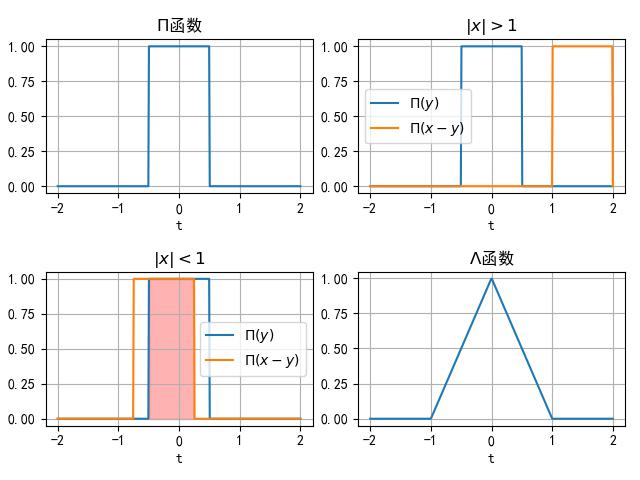
\includegraphics[width=0.8\textwidth]{conv}
    \caption{图解法求卷积示例}\label{fig:conv}
\end{figure}

初次接触卷积时,往往会对它的定义感到疑惑,因为在数学分析的课程中我们很少见到这
种“翻转、平移、相乘、积分”的结构。需要指出,卷积并不只有“时域相乘,频域卷积;
时域卷积,频域相乘”的物理意义,例如概率论中两连续型随机变量X,Y之和作为一种新的
随机变量Z,其概率密度函数$f_Z(z)$正是两个独立的随机变量的概率密度函数的卷积$f_X*f_Y(z)$.
类似于用“求曲线下方的面积”或“已知速度求位移”引入积分,尽管我们用一种较为自然的方
式引入了卷积,但不应该认为它只有单一的意义。不过,还是可以建立一些卷积的性质来
辅助我们理解卷积。

\noindent 1.卷积是一种起“平均化”作用的运算

给定区间$[a,b]$和权函数$w(x)$,$f(x)$的加权
均值为\[\frac{\int_{a}^{b}f(x)w(x)\,dx}{\int_{a}^{b}w(x)\,dx}\]给定$x$
时,$w(y)=g(x-y)$就是f的加权均值的倍数。进一步,卷积的光滑性高于用来卷积的两
个函数,并且在f可导时有$(f*g)'=f'*g$,因为
\[(f*g)'(x)=\frac{d}{dx}\int_{-\infty}^{\infty}f(x-y)g(y)\,dy=\int_{-\infty}^{\infty}f'(x-y)g(y)\,dy=f'*g\]

\noindent 2.卷积函数的支集

我们首先引入\textbf{支集}(support)的概念,读者只需理解其直观,真正理解它需要一些拓扑学的基础。设
$f:\mathbb{R}\to \mathbb{R}$\footnote{这里不对多元函数、复变函数等进行讨论,但读者容易自行推广这个定义。},f的\textbf{支集}
$supp\ f=\overline{\{x\in\mathbb{R}:f(x)\neq 0\}}$,这里上划线不是取共轭,
而是对集合取闭包,闭包包括集合本身的和它的极限点,$\mathbb{R}$中集合的闭包
是闭集,例如,$(a,b)$的闭包是$[a,b]$.集合$\{x\in\mathbb{R}:f(x)\neq 0\}$的提
出是自然的,取闭包则不那么容易理解。实际上,在度量空间(采用度量导出的拓扑)中,
一个集合是紧集(任给一个开区间组成的覆盖,总能从中取出有限覆盖)就等价于它是有
界闭集,描述有界区间的一种方式是说它是闭包紧的。因此,我们可以说在无穷远处为0的
函数有\textbf{紧支集}(compact support),对于p次连续可导的函数$f\in C^p(\mathbb{R})$,我们记
其中具有紧支集的函数空间为$C_0^p(\mathbb{R})$。至于引入这种术语的好处,则不属于本书的讨论范围。

卷积能够将两个函数的支集“相加”。设$supp f\in [a,b],supp g\in [c,d]$,则
$supp (f*g)\in [a+c,b+d]$,因为:
\begin{align*}
     & (f*g)(x) =\int_{-\infty}^{\infty}f(y)g(x-y)\,dy                               \\
     & \text{积分值非0}\Rightarrow y\in [a,b],x-y\in [c,d]\Leftrightarrow x\in [a+c,b+d]
\end{align*}

\noindent 3.函数变换下的卷积\\
(1)信号反转时的卷积:
\[(f^-)*(g^-)=(f*g)^-\]
\textbf{Proof:}
\begin{align*}
    (f^-)*(g^-)(x) & =\int_{-\infty}^{\infty}f^-(y)g^-(x-y)\,dy          \\
                   & =\int_{-\infty}^{\infty}f(-y)g(-(x-y))\,dy          \\
                   & =\int_{-\infty}^{\infty}f(z)g(-(x+z))(-dz) & (z=-y) \\
                   & =\int_{-\infty}^{\infty}f(z)g(-x-z)\,dz             \\
                   & =(f*g)^-(x)
\end{align*}
如果只有一个信号反转,则结果不再是卷积,而是f与g的互相关(在f,g都是实信号时),下面很
快将讨论它。

\noindent (2)信号时延、伸缩时的卷积

为了避免符号带来的误解,以后将
用$\tau$表示时延$\tau_b f(t)=f(t-b)$,用$\sigma$表示伸缩$\sigma_a f(t)=f(at)$
,并避免使用$\tau,\sigma$作为变量的符号。这样的做法在研究分布的性质时是必要的,
因为严格来讲不能给出分布的“自变量”,但例如$\delta$函数这样的分布又具有明显的
尺度变换的性质,见\ref{sec:distributions}.
\begin{align*}
    (\tau_b f)*g=\tau_b (f*g)=f*(\tau_b g) \\
    (\sigma_a f)*(\sigma_a g)=\frac{1}{|a|}\sigma_a(f*g)
\end{align*}
\textbf{Proof:}
\begin{align*}
    (\tau_b f)*g(x) & =\int_{-\infty}^{\infty}\tau_b f(y)g(x-y)\,dy           \\
                    & =\int_{-\infty}^{\infty}f(y-b)g(x-y)\,dy                \\
                    & =\int_{-\infty}^{\infty}f(z)g(x-(z+b))\,dz    & (z=y-b) \\
                    & =\int_{-\infty}^{\infty}f(z)g((x-b)-z)\,dz              \\
                    & =(f*g)(x-b)=\tau_b (f*g)(x)
\end{align*}
类似地,可以证明$f*(\tau_b g)=\tau_b (f*g)$.
\begin{align*}
    (\sigma_a f)*(\sigma_a g)(x) & =\int_{-\infty}^{\infty}\sigma_a f(y)\sigma_a g(x-y)\,dy                          \\
                                 & =\int_{-\infty}^{\infty}f(ay)g(a(x-y))\,dy                                        \\
                                 & =\frac{1}{|a|}\int_{-\infty}^{\infty}f(z)g(a x - z)\,dz  & (z=ay,dy=\frac{dz}{a}) \\
                                 & =\frac{1}{|a|}(f*g)(a x)=\frac{1}{|a|}\sigma_a(f*g)(x)
\end{align*}
和傅里叶变换的伸缩定理类似,这里也需要讨论a的正负,但不再赘述。

4.“面积”关系

我们已经提到,概率论中两个独立随机变量之和的概率密度函数是它们各自概率密度函数的卷积,这当
然要求两个概率密度函数在$\mathbb{R}$上的积分值为1时,它们的卷积在$\mathbb{R}$上的积
分值也为1。更一般地,如果$f,g\in L^1(\mathbb{R})$,则
\begin{align*}
    \int_{-\infty}^{\infty}(f*g)(x)\,dx & =\int_{-\infty}^{\infty}\,dx\int_{-\infty}^{\infty}f(y)g(x-y)\,dy                                   \\
                                        & =\int_{-\infty}^{\infty}f(y)\,dy\int_{-\infty}^{\infty}g(x-y)\,dx                                   \\
                                        & =\int_{-\infty}^{\infty}f(y)\,dy\int_{-\infty}^{\infty}g(u)\,du                           & (u=x-y) \\
                                        & =\left(\int_{-\infty}^{\infty}f(x)\,dx\right)\left(\int_{-\infty}^{\infty}g(x)\,dx\right)
\end{align*}

在统计学中,我们引入相关系数来描述两个随机变量之间的相关程度,类似地,在信号
处理中,我们引入\textbf{相关系数}(correlation coefficient)来描述两个信号之间的相关
程度。设$f,g\in L^2(\mathbb{R})$,它们的相关系数定义为
\begin{equation}
    \rho(f,g)=\frac{\langle f,g\rangle}{\|f\|\cdot\|g\|}
\end{equation}
其中$\langle f,g\rangle=\int_{-\infty}^{\infty}f(x)\overline{g(x)}dx$是$f$和
$g$的内积,$\|f\|=\sqrt{\langle f,f\rangle}$是$f$的范数。根据柯西-施瓦茨不等式,
相关系数的绝对值不超过1,且当且仅当$f$与$g$几乎处处成比例时取等,因此我们说,
$\rho(f,g)=\pm 1$时两信号\textbf{线性相关};$\rho(f,g)=0$时两信号\textbf{线性无关},
这相当于两函数正交。

有时信号之间存在时延差,这时我们可以定义\textbf{互相关}(cross-correlation)来描述它
们之间的相关程度。设$f,g\in L^2(\mathbb{R})$,它们的互相关定义为
\begin{equation}
    (f\star g)(x)=\int_{-\infty}^{\infty}f(y)\overline{g(x+y)}\,dy
\end{equation}
同样可以定义f的自相关$(f\star f)(x)$。互相关具有以下性质:
\begin{enumerate}
    \item $(f\star g) =f^-* \overline{g}=\overline{(g\star f)^-}$,如果$f,g$都是实信号,则$f\star g = (g\star f)^- =f^- *g=(f*g^-)^-$.
    \item $\mathcal{F} (f\star g) =\mathcal{F} f\overline{\mathcal{F} g}$,特别地,
          $\mathcal{F} (f\star f) =|\mathcal{F} f|^2$,这个结果称为\textbf{维纳-辛钦定理}(Wiener-Khinchin theorem)
    \item $f\star (\tau_b g)=\tau_{b} (f\star g)=(\tau_{-b}f)\star g$
    \item $(f\star g)\leq\|f\|\|g\|$,特别地,$(f\star f)(x)\leq (f\star f)(0)=\|f\|^2$
\end{enumerate}
\textbf{Proof:}
\begin{align*}
    1.(f\star g)(x)               & =\int_{-\infty}^{\infty}f(y)\overline{g(x+y)}\,dy                                                                   \\
                                  & =\int_{-\infty}^{\infty}f(-y)\overline{g(x-y)}\,dy                                                                  \\
                                  & =\int_{-\infty}^{\infty}f^-(y)\overline{g(x-y)}\,dy                                                                 \\
                                  & = (f^- * \overline{g})(x)                                                                                           \\
    (f\star g)(x)                 & =\int_{-\infty}^{\infty}f(y)\overline{g(x+y)}\,dy                                                                   \\
                                  & =\overline{\int_{-\infty}^{\infty}g(x+y)\overline{f(y)}\,dy}                                                        \\
                                  & =\overline{(g\star f)(-x)}=\overline{(g\star f)^-(x)}                                                               \\
    2.\mathcal{F} (f\star g)(\xi) & =\int_{-\infty}^{\infty}(f\star g)(x)e^{-2\pi i\xi x}\,dx                                                           \\
                                  & =\int_{-\infty}^{\infty}e^{-2\pi i\xi x}\,dx\int_{-\infty}^{\infty}f(y)\overline{g(x+y)}\,dy                        \\
                                  & =\iint\limits_{\mathbb{R}^2}f(y)\overline{g(x+y)}e^{-2\pi i\xi x}\,dy\,dx                                           \\
                                  & =\int_{-\infty}^{\infty}f(y)\,dy\int_{-\infty}^{\infty}\overline{g(x+y)}e^{-2\pi i\xi x}\,dx                        \\
                                  & =\int_{-\infty}^{\infty}f(y)e^{2\pi i\xi y}\,dy\int_{-\infty}^{\infty}\overline{g(u)}e^{-2\pi i\xi u}\,du & (u=x+y) \\
                                  & =\mathcal{F} f(\xi)\overline{\mathcal{F} g(\xi)}
\end{align*}这里不涉及频率、角频率的问题,读者可以自行验证。
\begin{align*}
    3.(f\star (\tau_b g))(x)  & =\int_{-\infty}^{\infty}f(y)\overline{(\tau_b g)(x+y)}\,dy                                                  \\
                              & =\int_{-\infty}^{\infty}f(y)\overline{g(x+y-b)}\,dy                                                         \\
                              & =(f\star g)(x-b)=\tau_{b} (f\star g)(x)                                                                     \\
    ( (\tau_{-b}f)\star g)(x) & =\int_{-\infty}^{\infty}(\tau_{-b}f)(y)\overline{g(x+y)}\,dy                                                \\
                              & =\int_{-\infty}^{\infty}f(y+b)\overline{g(x+y)}\,dy                                                         \\
                              & =\int_{-\infty}^{\infty}f(z)\overline{g(x+z-b)}\,dz                                               & (z=y+b) \\
                              & =(f\star g)(x-b)=\tau_{b} (f\star g)(x)                                                                     \\
    4. (f\star g)(x)          & =\int_{-\infty}^{\infty}f(y)\overline{g(x+y)}\,dy                                                           \\
                              & \leq \sqrt{\int_{-\infty}^{\infty}|f(y)|^2\,dy\int_{-\infty}^{\infty}|\overline{g(x+y)}|^2\,dy  }           \\
                              & =\sqrt{\|f\|^2\|g\|^2}=\|f\|\cdot\|g\|                                                                      \\
\end{align*}

对于功率信号$f,g$,定义互相关函数为
\begin{equation}
    (f\star g)(x)=\lim_{T\to\infty}\frac{1}{2T}\int_{-T}^{T}f(y)\overline{g(x+y)}\,dy
\end{equation}
其性质不再单独讨论。

一些文献也将互相关函数定义为$R_{fg}(x)=\int_{-\infty}^{\infty}f(y)\overline{g(x-y)}\,dy=\int_{-\infty}^{\infty}f(x+y)g(y)\,dy$
,功率信号同理,这与上面讨论的互相关没有本质区别。

\section{分布及其傅里叶变换}\label{sec:distributions}

经典的数学分析理论难以处理单位阶跃函数的导数,也无法对一些比较比基本的函数如正弦
、余弦函数做傅里叶变换,甚至因此傅里叶反演公式不总是成立(注意我们之前仅在形式上
使用傅里叶反演公式),要扩充这个理论,标准的做法是引入\textbf{广义函数}(gerneralized function)
,又称\textbf{分布}(distribution)\footnote{事实上这个名称更泛用一些。}。分布
这个名称一开始是由物理学家引入的,例如在描述点电荷的分布时,经典函数是失效的,于
是在20世纪20年代末到30年代初,狄拉克及一众物理学家开始用分布进行运算,到30年代
中,索伯列夫首先明确提出了广义函数的思想,后于40年代末由施瓦兹发展,他因这一工作
获得1950年的菲尔兹奖。因此,下面将提到的广义函数空间$\mathcal{D} $也称为
\textbf{索伯列夫-施瓦兹广义函数空间}。

下面首先对一般的分布理论做一些讨论,再转回傅里叶分析中对于分布的应用,这时不对
严谨性做过多要求,希望了解它们的读者可以参考泛函分析或傅里叶分析的教材。我们先介
绍\textbf{泛函} (functioinal)和\textbf{对偶空间}(dual space)的概念。

设X和Y是同一数域上的线性空间(这里不妨设为$\mathbb{R}$)如果
$\forall x_1,x_2\in X$,映射$A:X\to Y$满足
\begin{align*}
    A(x_1)+A(x_2) & =A(x_1+x_2)                        \\
    A(\lambda x)  & =\lambda A(x),\lambda\in\mathbb{R}
\end{align*}
则称A是\textbf{线性映射}。特别地,如果Y是一个数域(例如$\mathbb{R,C}$),则
将A称为\textbf{线性函数};如果X还是某种函数空间,则将A称为\textbf{线性泛函}。
例如,$A:C([a,b],\mathbb{R})\to\mathbb{R},A(f):=f(x_0)$和$A:C([a,b],\mathbb{R})\to\mathbb{R},A(f):=\int_{a}^{b}f(x)\,dx$
都是线性泛函。有时,我们不区分X究竟是不是函数空间,而统一地把线性函数称为线性泛
函。

给定一个实线性空间V,它的\textbf{对偶空间}是V上所有线性函数$A:V\to\mathbb{R}$
构成的线性空间(读者可以自行定义线性函数的加法和数乘,并验证它是线性空间),记
为$\mathcal{L} (V;\mathbb{R})$或$V^*$。对有限维线性空间,它的对偶空间与它本身的维数
相同,因为定义V上的线性函数就等价于对V的一组基定义线性函数;对于无限维线性空间
,它的对偶空间也是无限维的。

我们已经看到,分布(例如狄拉克$\delta$)难以用经典的“函数”来描述,这时我们可以
考察它们与一系列\textbf{检验函数}(test function)$\varphi$的作用,具体来说,记$\mathbb{R}$
上的复值光滑紧支函数集为$\mathcal{C} $,如果将检验函数集取为$\mathcal{C}$,我们
将其对偶空间$\mathcal{D} $中的元素称为分布,并规定函数$f\in \mathcal{C} $
\footnote{实际上这里不需要要求$f\in\mathcal{C} $,只需要f在$\mathbb{R}$上局部可积(在任
    意闭区间上可积)即可,但为了简化讨论,我们仅考虑光滑紧支函数。}所产生的分布$T_f$
为作用在$\mathcal{C}$上的以下\textbf{泛函}:
\begin{equation}
    \langle T_f,\varphi\rangle:=\int_{-\infty}^{\infty}f(x)\varphi(x)\,dx,\varphi\in\mathcal{C}
\end{equation}
将这样的分布称为\textbf{正则分布},而将无法用紧支函数描述的分布称为\textbf{奇异分布}。
例如,尽管我们从形式上给出了$\delta$函数的定义,但它实际上应该采用定义
\[\langle \delta,\varphi\rangle:=\delta(\varphi):=\varphi(0)\]
容易验证这与我们一开始给出的$\delta$作为“函数”的性质是相符的:
\[\langle \delta,\varphi\rangle=\int_{-\infty}^{\infty}\delta(x)\varphi(x)\,dx=\int_{-\infty}^{\infty}\delta(x)\varphi(0)\,dx=\varphi(0)\]

下面来定义分布与函数的乘法和分布的导数。这一部分中,我们的原则是:\textbf{奇异分布与正
    则分布具有相同的性质},换言之,只要能够对正则分布定义的算子,就能够对奇异分布
做相同的定义。在讨论分布的傅里叶变换时,还将定义更多的算子,例如分布卷积、尺度变换等。

设$f,g,\varphi\in\mathcal{C} $,有
\begin{align*}
    \langle (f\cdot g),\varphi\rangle=\int_{-\infty}^{\infty}(f\cdot g)(x)\varphi(x)\,dx=\int_{-\infty}^{\infty}f(x)(g\cdot\varphi)(x)\,dx=\langle f,(g\cdot\varphi)\rangle
\end{align*}
因此对于任意的分布$T\in\mathcal{D} $,定义它与$g\in\mathcal{C} $的乘积$gT$
由以下等式给出:
\begin{equation}
    \langle gT,\varphi\rangle=\langle T,g\varphi\rangle
\end{equation}
$g\varphi$就是普通的函数乘法。现在就可以说,分布集$\mathcal{D} $构成函数环
$\mathcal{C} $上的模(module),并且可以验证$\delta$的取样性质:
\begin{align*}
     & \langle g\delta,\varphi\rangle=\langle \delta,g\varphi\rangle=g(0)\varphi(0)=g(0)\langle\delta,\varphi\rangle \Rightarrow  g\delta=g(0)\delta
\end{align*}

用同样的思路定义分布的微分:设$f,g,\varphi\in\mathcal{C} $,有
\begin{align*}
    \langle f',\varphi\rangle=\int_{-\infty}^{\infty}f'(x)\varphi(x)\,dx=-\int_{-\infty}^{\infty}f(x)\varphi'(x)\,dx=\langle f,\varphi'\rangle
\end{align*}
因此
\begin{equation}
    \langle T',\varphi\rangle=-\langle T,\varphi'\rangle
\end{equation}
注意$\varphi\in\mathcal{C} $是无限阶可导的,我们可以由此定义分布的任意阶导数,
例如\ref{sec:signal}中提到的单位阶跃函数$u(t)$和$\delta$,现在就可以将它们
视为分布并求各阶导数:
\begin{align*}
     & \langle u,\varphi\rangle:=\int_{0}^{\infty}\varphi(x)\,dx                                                                      \\
     & \langle u',\varphi\rangle=-\langle u,\varphi'\rangle=-\int_{0}^{\infty}\varphi'(x)\,dx=\varphi(0)=\langle\delta,\varphi\rangle \\
     & \langle \delta',\varphi\rangle=-\langle \delta,\varphi'\rangle=-\varphi'(0)
\end{align*}
$\delta$的高阶导数可以依此类推,它们已经难以用类似$\delta(x)$的“函数”描述,但
可以看到$\delta^{(n)}$作为一个泛函(分布)作用是取测试函数的$(-1)^n$倍的n阶导。
现在也就不难理解$\delta^{(n)}$与函数相乘的公式,例如,
\begin{align*}
    \langle g\delta',\varphi\rangle & =\langle \delta',g\varphi\rangle                \\
                                    & =-\langle\delta,(g\varphi)'\rangle              \\
                                    & =-\langle\delta,g'\varphi+g\varphi'\rangle      \\
                                    & =-(g(0)\varphi'(0)+g'(0)\varphi(0))             \\
                                    & =\langle g(0)\delta'-g'(0)\delta,\varphi\rangle
    \Rightarrow g\delta'=g(0)\delta'-g'(0)\delta
\end{align*}

现在指出分布的微分运算的某些性质。
\begin{enumerate}
    \item 任何分布$T\in\mathcal{D} $都是无穷次可微的
    \item 微分算子$D:\mathcal{D} \to\mathcal{D} $是线性的
    \item 微分算子D满足莱布尼兹法则(Leibniz rule):
          \[(gT)'=g'T+gT'\]从而数学分析中的莱布尼兹公式在分布理论中仍成立:
          \[(gT)^{(m)}=\sum_{k=0}^{m}C_m^k T^{(k)}g^{m-k}\]
    \item 微分算子D是连续的(表述见证明)
\end{enumerate}
\textbf{Proof:}\begin{enumerate}
    \item 得自$\mathcal{C} $中函数的无限可微性:$\langle T^{(m)},\varphi\rangle=(-1)^m\langle T,\varphi^{(m)}\rangle$.
    \item 显然。
    \item 只需验证莱布尼兹法则。
          \begin{align*}
              \langle (gT)',\varphi\rangle & =-\langle gT,\varphi'\rangle=-\langle T,g\varphi'\rangle=-\langle T,(g\varphi)'-g'\varphi\rangle                                            \\
                                           & =\langle T',g\varphi\rangle+\langle T,g'\varphi\rangle=\langle gT',\varphi\rangle+\langle g'T,\varphi\rangle=\langle gT'+g'T,\varphi\rangle
          \end{align*}
    \item 设当$m\to\infty$时,$T_m\to T$,即$\forall\varphi\in\mathcal{C} ,\langle T_m,\varphi\rangle\to\langle T,\varphi\rangle$,
          则\[\langle T_m',\varphi\rangle=-\langle T_m,\varphi'\rangle\to-\langle T,\varphi'\rangle=\langle T',\varphi\rangle\]
\end{enumerate}
可以看到,分布理论中极限的概念是通过测试函数来定义的,如果分布序列$\{T_m\}_{m=1}^{\infty}$
作用在任何测试函数上都是趋于某个分布T作用于这个测试函数的值,就说序列$\{T_m\}$
\textbf{弱收敛}(converge weakly)于T,并记为$T_m\to T$。

接下来讨论分布理论在傅里叶分析中的应用。我们的目标是,在这个新的理论体系下:
\begin{itemize}
    \item 允许$\delta$信号,单位阶跃信号,多项式,正弦、余弦函数等信号(作为分布)做傅里叶变换
    \item 傅里叶变换和其反变换同时有定义傅里叶反演公式成立
    \item 帕塞瓦尔恒等式成立
\end{itemize}
我们将看到,分布$T$的傅里叶变换$\mathcal{F} T$定义为
\begin{equation}
    \langle\mathcal{F}T,\varphi\rangle=\langle T,\mathcal{F}\varphi\rangle
\end{equation}
然而,测试函数$\varphi\in\mathcal{C} $的傅里叶变换$\mathcal{F}\varphi$并不属于
$\mathcal{C} $
(关于这一点的说明,以及施瓦兹函数类的引出,见附录\ref{sec:Schwartz_Functions})
,这说明测试函数集$\mathcal{C} $在傅里叶分析中的表现不够好,我们需要引入新的测试函数空间,以保证
$\mathcal{F}\varphi$仍然是测试函数。这个测试函数空间正是\textbf{施瓦兹空间}(Schwartz space)$\mathcal{S} $
,它是$\mathbb{R}$上所有无限可微函数的集合,这些函数及其各阶导数都以比任何负幂更快的速度趋于0,即
\[\mathcal{S} =\{\varphi\in C^{\infty}(\mathbb{R} ):\lim_{|x|\to\infty}|x|^m\varphi^{(n)}(x)=0,\forall m,n\in\mathbb{N} \}\]
施瓦兹空间中的函数称为\textbf{施瓦兹函数}(Schwartz function),它们是非常光滑且
衰减很快的函数,因此又称为\textbf{速降函数}(rapidly decreasing function),例
如高斯函数$e^{-x^2}$及其各阶导数都属于施瓦兹空间。施瓦兹空间的对偶空间
$\mathcal{T} :=\mathcal{S}^*$中的元素称为\textbf{施瓦兹分布}(Schwartz distribution)
或\textbf{缓增分布}(tempered distribution)。我们仍定义
\begin{align}
    T(\varphi)                 & =\langle T,\varphi\rangle                                        \\
    \langle T_f,\varphi\rangle & =\int_{-\infty}^{\infty}f(x)\varphi(x)\,dx,\varphi\in\mathcal{S}
\end{align}
易见$\mathcal{C} \subset \mathcal{S} ,\mathcal{T} \subset\mathcal{D}. $

有了施瓦兹函数类$\mathcal{S} $和缓增分布$\mathcal{T} $,我们就可以定义分布的傅里
叶变换,还可以定义有关分布的一系列算子。前文中曾定义分布与函数的乘法和分布的导数,
现在认为正则分布是由施瓦兹函数导出的,则显然能够推广到缓增分布,即\begin{align}
    \langle gT,\varphi\rangle=\langle T,g\varphi\rangle,\langle T',\varphi\rangle=\langle T,\varphi'\rangle,g\in\mathcal{S} ,T\in\mathcal{T}
\end{align}
用同样的方式,我们依次讨论作用于缓增分布的各种算子。

\noindent 1.傅里叶变换

设$f,\varphi\in\mathcal{S} ,T_f\in\mathcal{T} $,则
\begin{align*}
    \langle\mathcal{F}T_f,\varphi\rangle & =\int_{-\infty}^{\infty}\mathcal{F}f(x)\varphi(x)\,dx                                       \\
                                         & =\int_{-\infty}^{\infty}\varphi(x)\,dx\int_{-\infty}^{\infty}f(y)e^{-2\pi ixy}\,dy          \\
                                         & =\int_{-\infty}^{\infty}f(y)\,dy\int_{-\infty}^{\infty}\varphi(x)e^{-2\pi ixy}\,dx          \\
                                         & =\int_{-\infty}^{\infty}f(y)\mathcal{F}\varphi(y)\,dy=\langle T_f,\mathcal{F}\varphi\rangle
\end{align*}
因此我们定义分布的傅里叶变换为
\begin{equation}
    \langle\mathcal{F}T,\varphi\rangle=\langle T,\mathcal{F}\varphi\rangle,T\in\mathcal{T} ,\varphi\in\mathcal{S}
\end{equation}

傅里叶逆变换同理。只要承认函数的傅里叶反演公式,分布的傅里叶反演公式就自然成立:
\begin{align*}
    \langle \mathcal{F} ^{-1}\mathcal{F} T,\varphi\rangle&=\langle \mathcal{F} T,\mathcal{F} ^{-1}\varphi\rangle\\
    &=\langle T,\mathcal{F} \mathcal{F} ^{-1}\varphi\rangle\\
    &=\langle T,\varphi\rangle\\
    \langle \mathcal{F} \mathcal{F} ^{-1}T,\varphi\rangle&=\langle T,\mathcal{F} ^{-1}\mathcal{F} \varphi\rangle\\
    &=\langle T,\varphi\rangle
\end{align*}

线性性依然成立。尽管没有明确指出,我们也会很自然的想到定义
\begin{equation}
    \langle aT+bS,\varphi\rangle=a\langle T,\varphi\rangle+b\langle S,\varphi\rangle
\end{equation}
于是\begin{align*}
    \langle \mathcal{F} (aT+bS),\varphi\rangle & =a\langle T,\mathcal{F} \varphi\rangle+b\langle S,\mathcal{F} \varphi\rangle                     \\
                                               & =a\langle \mathcal{F} T,\varphi\rangle+b\langle \mathcal{F} S,\varphi\rangle                     \\
                                               & =\langle a\mathcal{F} T+b\mathcal{F} S,\varphi\rangle                                            \\
                                               & \Rightarrow \mathcal{F} (aT+bS)=a\mathcal{F} T+b\mathcal{F} S,a,b\in\mathbb{C},S,T\in\mathcal{T}
\end{align*}

\noindent 例5.1.现在可以严谨地求出$\delta$的傅里叶变换:
\begin{align*}
    \langle\mathcal{F}\delta,\varphi\rangle=\langle \delta,\mathcal{F}\varphi\rangle=\mathcal{F}\varphi(0)=\int_{-\infty}^{\infty}\varphi(x)\,dx=\langle \mathds{1},\varphi\rangle \\
    \Rightarrow\mathcal{F}\delta =\mathds{1}
\end{align*}
例5.2.$\delta$的平移$\delta_a$作为一种分布,定义为
\begin{equation}
    \delta_a(\varphi)=\langle \delta_a,\varphi\rangle=\varphi(a)
\end{equation}
它的傅里叶变换为
\lr{
\langle\mathcal{F}\delta_a,\varphi\rangle&=\langle \delta_a,\mathcal{F}\varphi\rangle\\
&=\mathcal{F}\varphi(a)\\
&=\int_{-\infty}^{\infty}\varphi(x)e^{-2\pi iax}\,dx\\
&=\langle e^{-2\pi iax},\varphi\rangle \\
&\Rightarrow\mathcal{F}\delta_a =e^{-2\pi iax}
}{
\langle\mathcal{F}\delta_a,\varphi\rangle&=\langle \delta_a,\mathcal{F}\varphi\rangle\\
&=\mathcal{F}\varphi(a)\\
&=\int_{-\infty}^{\infty}\varphi(x)e^{-i a x}\,dx\\
&=\langle e^{-i a x},\varphi\rangle \\
&\Rightarrow\mathcal{F}\delta_a =e^{-i a x}
}
根据阿贝尔-狄利克雷判别法(A-D判别法,请自行查看数学分析的教材),$\langle e^{-i a x},\varphi\rangle$
是有意义的。可以看出这与函数的傅里叶变换的平移定理很相似,我们将在后面给出分布的平移、伸缩,并由
此得到一些分布的傅里叶变换的性质。

\noindent 例5.3.分布$\mathds{1}$的傅里叶变换:尽管$\mathds{1}\notin L^1(\mathbb{R})$,但可以
认为它是缓增分布,因为对于任意的$\varphi\in\mathcal{S} $,都有
\[\langle \mathds{1},\varphi\rangle=\int_{-\infty}^{\infty}\varphi(x)\,dx<\infty\]
因此可以求它的傅里叶变换:
\lr{
    \langle \mathcal{F} \mathds{1},\varphi&=\langle \mathds{1},\mathcal{F} \varphi\rangle\\
    &=\int_{-\infty}^{\infty}\mathcal{F} \varphi(\xi)\,d\xi\\
    &=\mathcal{F} \mathcal{F} \varphi(0)\\
    &=\varphi(0)=\langle \delta,\varphi\rangle\\
    \Rightarrow \mathcal{F} \mathds{1}&=\delta
}{
    \langle \mathcal{F} \mathds{1},\varphi\rangle&=\langle \mathds{1},\mathcal{F} \varphi\rangle\\
    &=\int_{-\infty}^{\infty}\mathcal{F} \varphi(\xi)\,d\xi\\
    &=\mathcal{F} \mathcal{F} \varphi(0)\\
    &=2\pi\varphi(0)=2\pi\langle \delta,\varphi\rangle\\
    \Rightarrow \mathcal{F} \mathds{1}&=2\pi\delta
}

\noindent 2.分布的反转

设$f,\varphi\in\mathcal{S} ,T_f\in\mathcal{T} $,自然可以定义$T_f^-=T_{f^-}$,
\begin{align*}
    \langle T_f^-,\varphi\rangle & =\int_{-\infty}^{\infty}f(-x)\varphi(x)\,dx \\
                                 & =\int_{-\infty}^{\infty}f(y)\varphi(-y)\,dy \\
                                 & =\langle T_f,\varphi^-\rangle
\end{align*}
因此我们定义分布的反转为
\begin{equation}
    \langle T^-,\varphi\rangle=\langle T,\varphi^-\rangle,T\in\mathcal{T} ,\varphi\in\mathcal{S}
\end{equation}
有了反转就可以定义分布的奇偶性:如果$T^-=T$,则称T为\textbf{偶分布};如果$T^-=-T$
,则称T为\textbf{奇分布}。

从施瓦兹函数的傅里叶变换的对偶性,就能得到缓增分布的傅里叶变换的对偶性:
\begin{align*}
    \langle\mathcal{F}(T^-),\varphi\rangle=\langle T^-,\mathcal{F}\varphi\rangle=\langle T,\mathcal{F} \varphi^-\rangle=\langle\mathcal{F}T,\varphi^-\rangle=\langle(\mathcal{F}T)^-,\varphi\rangle \\
    \Rightarrow\mathcal{F}(T^-)= (\mathcal{F}T)^-
\end{align*}
和常规的函数一样,现在也可以不区分反转与傅里叶变换的先后,而统一地记作$\mathcal{F} T^-$.
考察反转与傅里叶逆变换的关系:
\lr{
    \langle\mathcal{F}T^-,\varphi\rangle=\langle T,\mathcal{F}\varphi^-\rangle=\langle T,\mathcal{F} ^{-1}\varphi\rangle=\langle\mathcal{F}^{-1}T,\varphi\rangle\\
    \Rightarrow\mathcal{F}T^-= \mathcal{F}^{-1}T
}{
    \langle\mathcal{F}T^-,\varphi\rangle=\langle T,\mathcal{F}\varphi^-\rangle=\langle T,2\pi\mathcal{F} ^{-1}\varphi\rangle=2\pi\langle\mathcal{F}^{-1}T,\varphi\rangle\\
    \Rightarrow\mathcal{F}T^-= 2\pi\mathcal{F}^{-1}T
}
这与前文中函数的傅里叶变换对偶性完全一样。有了对偶性,就可以得到\textbf{帕塞瓦尔恒等式}
(Parceval's identity):\lr{
    \int_{-\infty}^{\infty}|f(t)|^2\,dt=\int_{-\infty}^{\infty}|\mathcal{F} f(\xi)|^2\,d\xi
}{
    \int_{-\infty}^{\infty}|f(t)|^2\,dt=\frac{1}{2\pi}\int_{-\infty}^{\infty}|\mathcal{F} f(\omega)|^2\,d\omega
}
\textbf{Proof:}设$f,g\in\mathcal{S} $,\lr{
    \langle \mathcal{F} f,\overline{\mathcal{F} g}\rangle&=\langle \mathcal{F} f,\mathcal{F}^{-1}\overline{g}\rangle\\
    &=\langle f,\mathcal{F} \mathcal{F} ^{-1}\overline{g}\rangle\\
    &=\langle f,\overline{g}\rangle
}{
    \langle \mathcal{F} f,\overline{\mathcal{F} g}\rangle&=\langle f,2\pi\mathcal{F}^{-1}\overline{g}\rangle\\
    &=\langle f,2\pi\mathcal{F} \mathcal{F} ^{-1}\overline{g}\rangle\\
    &=2\pi\langle f,\overline{g}\rangle
}
取$g=f$即证,尽管限制了函数的范围,但这个证明比前文中积分换序的证明简洁得多。

例5.14.$\delta$是偶分布:
\begin{align*}
    \langle \delta^-,\varphi\rangle & =\langle \delta,\varphi^-\rangle=\varphi^-(0)=\varphi(0)=\langle \delta,\varphi\rangle \\
    \Rightarrow \delta^-            & =\delta
\end{align*}
例5.5.应用对偶性求$\mathds{1}$的傅里叶逆变换:
\lr{
    \mathcal{F} \mathds{1}=\mathcal{F} ^{-1}\mathds{1}^-=\delta^-=\delta
}{
    \mathcal{F} \mathds{1}=2\pi\mathcal{F} ^{-1}\mathds{1}^- =2\pi\delta^- =2\pi\delta
}
\noindent 例5.6.复指数函数$e^{iat}$的傅里叶变换:作为函数当然不能求$e^{iat}$的傅里叶变换,
我们甚至无法确定它在0处的傅里叶变换:$\int_{-\infty}^{\infty}e^{iat}\,dt$不存在。
但它可以视为一个缓增分布,前文中已经提到$\langle e^{iat},\varphi\rangle$是收敛
的。下面应用对偶性求它的傅里叶变换:
\lr{
\mathcal{F} [e^{2\pi iat}]=\mathcal{F}^{-1}[e^{2\pi iat}]^-=\delta_{a}^-=\delta_{-a}
}{
\mathcal{F} [e^{iat}]=2\pi\mathcal{F}^{-1}[e^{iat}]^- =2\pi\delta_{a}^- =2\pi\delta_{-a}
}
请读者自行验证$\delta_{a}^-= \delta_{-a}$.

\noindent 例5.7.正弦、余弦函数的傅里叶变换:根据欧拉公式$e^{ix}=\cos(x)+i\sin(x)$,
有\[\cos(x)=\frac{e^{ix}+e^{-ix}}{2},\sin(x)=\frac{e^{ix}-e^{-ix}}{2i}\]因此
\lr{
    \mathcal{F} [\cos(2\pi ax)]=\frac{1}{2}(\mathcal{F} [e^{2\pi iax}]+\mathcal{F} [e^{-2\pi iax}])=\frac{1}{2}(\delta_{-a}+\delta_{a}) \\
    \mathcal{F} [\sin(2\pi ax)]=\frac{1}{2i}(\mathcal{F} [e^{2\pi iax}]-\mathcal{F} [e^{-2\pi iax}])=\frac{1}{2i}(\delta_{-a}-\delta_{a})
}{
    \mathcal{F} [\cos(ax)]=\frac{1}{2}(\mathcal{F} [e^{iax}]+\mathcal{F} [e^{-iax}])=\pi(\delta_{-a}+\delta_{a}) \\
    \mathcal{F} [\sin(ax)]=\frac{1}{2i}(\mathcal{F} [e^{iax}]-\mathcal{F} [e^{-iax}])=-i\pi(\delta_{-a}-\delta_{a})
}

\noindent 3.分布的共轭

设$f,\varphi\in\mathcal{S} ,T_f\in\mathcal{T} $,则
\begin{align*}
    \langle \overline{T_f},\varphi\rangle & =\overline{\langle T_f,\overline{\varphi}\rangle}=\overline{\int_{-\infty}^{\infty}f(x)\overline{\varphi(x)}\,dx}=\overline{\langle T_f,\overline{\varphi}\rangle} \\
\end{align*}
因此我们定义分布的共轭为
\begin{equation}
    \langle \overline{T},\varphi\rangle=\overline{\langle T,\overline{\varphi}\rangle},T\in\mathcal{T} ,\varphi\in\mathcal{S}
\end{equation}
有了共轭就可以定义实分布和虚分布:如果$\overline{T}=T$,则称T为\textbf{实分布};如果
$\overline{T}=-T$,则称T为\textbf{纯虚分布}。现在就来考察最后一条对偶性:
\begin{align*}
    \langle\mathcal{F}T^-,\varphi\rangle =\langle T,\mathcal{F}\varphi^-\rangle
\end{align*}
我们并不能保证$\varphi$是实值函数\footnote{尽管在原始定义中没有提到这一点,但和前
    面引入施瓦兹函数类一样,要保证施瓦兹函数的傅里叶变换仍然是施瓦兹函数,而实值函数的
    傅里叶变换往往是复值函数。},因此并不能推出实分布的最后一条对偶性。不过,我们还是可
以得到分布的傅里叶变换的对称性:
\begin{align*}
    T^-=T\Rightarrow\mathcal{F} T^-=\mathcal{F} T \\
    T^-=-T\Rightarrow\mathcal{F} T^-=-\mathcal{F} T
\end{align*}
因此分布的傅里叶变换的奇偶性与分布本身相同。

\noindent 4.分布的平移和伸缩

设$f,\varphi\in\mathcal{S} ,T_f\in\mathcal{T} $,自然可以定义$\tau_b T_f=T_{\tau_b f}$,
\begin{align*}
    \langle \tau_b T_f,\varphi\rangle & =\int_{-\infty}^{\infty}f(x-b)\varphi(x)\,dx \\
                                      & =\int_{-\infty}^{\infty}f(y)\varphi(y+b)\,dy \\
                                      & =\langle T_f,\tau_{-b}\varphi\rangle
\end{align*}
因此我们定义分布的平移为
\begin{equation}
    \langle \tau_b T,\varphi\rangle=\langle T,\tau_{-b}\varphi\rangle,T\in\mathcal{T} ,\varphi\in\mathcal{S}
\end{equation}
设$f,\varphi\in\mathcal{S} ,T_f\in\mathcal{T} $,自然可以定义$\sigma_a T_f=T_{f(ax)}$,
\begin{align*}
    \langle \sigma_a T_f,\varphi\rangle & =\int_{-\infty}^{\infty}f(ax)\varphi(x)\,dx                                  \\
                                        & =\frac{1}{|a|}\int_{-\infty}^{\infty}f(y)\varphi\left(\frac{y}{a}\right)\,dy \\
                                        & =\frac{1}{|a|}\langle T_f,\sigma_{1/a}\varphi\rangle
\end{align*}
因此我们定义分布的伸缩为
\begin{equation}
    \langle\sigma_a T,\varphi\rangle=\langle T,\frac{1}{|a|}\sigma_{1/a}\varphi\rangle,T\in\mathcal{T} ,\varphi\in\mathcal{S}
\end{equation}

现在就可以建立分布的傅里叶变换的平移和尺度变换定理:
\begin{align*}
    \langle\mathcal{F}(\tau_b T),\varphi\rangle =\langle \tau_b T,\mathcal{F}\varphi\rangle=\langle T,\tau_{-b}\mathcal{F}\varphi\rangle=\langle T,e^{2\pi ibx}\mathcal{F}\varphi\rangle=\langle \mathcal{F}(e^{2\pi ibx}T),\varphi\rangle \\
    \Rightarrow\mathcal{F}(\tau_b T)           =\mathcal{F}(e^{2\pi ibx}T)
\end{align*}
\begin{align*}
    \langle\mathcal{F}(\sigma_a T),\varphi\rangle =\langle \sigma_a T,\mathcal{F}\varphi\rangle=\langle T,\frac{1}{|a|}\sigma_{\frac{1}{a}}\mathcal{F}\varphi\rangle=\langle T,\frac{1}{|a|}\mathcal{F}\sigma_a \varphi\rangle=\langle \frac{1}{|a|}\mathcal{F}(\sigma_a T),\varphi\rangle \\
    \Rightarrow\mathcal{F}(\sigma_a T)           =\frac{1}{|a|}\mathcal{F}(\sigma_a T)
\end{align*}

\noindent 5.分布的傅里叶变换的微分性质

我们已经得到$\langle T',\varphi\rangle=-\langle T,\varphi'\rangle$,现在结合
分布与函数的乘法,仿照函数的情形得到分布的傅里叶变换的微分性质:
\lr{
    \langle\mathcal{F} (T'),\varphi\rangle&=-\langle T,(\mathcal{F} \varphi)'\rangle\\
    &=\langle T,\mathcal{F} (2\pi i t\varphi)\rangle\\
    &=\langle 2\pi i\xi\mathcal{F}T,\varphi\rangle\\
    &\Rightarrow\mathcal{F} (T')=2\pi i\xi\mathcal{F}T
}{
    \langle\mathcal{F} (T'),\varphi\rangle&=-\langle T,(\mathcal{F} \varphi)'\rangle\\
    &=\langle T,\mathcal{F} (i t\varphi)\rangle\\
    &=\langle i\omega\mathcal{F}T,\varphi\rangle\\
    &\Rightarrow\mathcal{F} (T')=i\omega\mathcal{F}T
}
这与函数的傅里叶变换的微分性质一致,注意将$t$换成$\xi$或$\omega$,只是符号上的改
变,用以区分所讨论的场景。同样地,
\lr{
    \langle (\mathcal{F} T)',\varphi\rangle&=\langle T,-\mathcal{F} (\varphi')\rangle\\
    &=\langle T,-2\pi i\xi\mathcal{F} \varphi\rangle\\
    &=\langle -\mathcal{F} (2\pi i tT),\varphi\rangle\\
    &\Rightarrow (\mathcal{F} T)'=-\mathcal{F} (2\pi i tT)
}{
    \langle(\mathcal{F} T)',\varphi\rangle&=\langle T,-\mathcal{F} (\varphi)'\rangle\\
    &=\langle T,-i\omega\mathcal{F} \varphi\rangle\\
    &=\langle -\mathcal{F} (itT),\varphi\rangle\\
    &\Rightarrow (\mathcal{F} T)'=-\mathcal{F} (itT)
}
也即
\lr{
    \mathcal{F} (tT)=\frac{i}{2\pi}(\mathcal{F} T)'
}{
    \mathcal{F} (tT)=i(\mathcal{F} T)'
}

\noindent 6.分布的卷积

设$f,g,\varphi\in\mathcal{S} ,T_f\in\mathcal{T} $,自然可以定义$(T_f)*g=T_{(f*g)}$,
\begin{align*}
    \langle T_f*g,\varphi\rangle & =\int_{-\infty}^{\infty}(f*g)(x)\varphi(x)\,dx                                                      \\
                                 & =\int_{-\infty}^{\infty}\left(\int_{-\infty}^{\infty}f(y)g(x-y)\,dy\right)\varphi(x)\,dx            \\
                                 & =\int_{-\infty}^{\infty}f(y)\,dy\int_{-\infty}^{\infty}g(x-y)\varphi(x)\,dx                         \\
                                 & =\int_{-\infty}^{\infty}f(y)\,dy\int_{-\infty}^{\infty}g^- (y-x)\varphi(x)\,dx                      \\
                                 & =\int_{-\infty}^{\infty}f(y)[(g^-) *\varphi](y)\,dy                                                 \\
                                 & =\langle T_f,(g^-)*\varphi\rangle                                                                   \\
                                 & \Rightarrow \langle T*g,\varphi\rangle=\langle T,(g^-)*\varphi\rangle
\end{align*}

从定义分布与函数的卷积的过程可以看出,应当要求卷积的交换律仍然成立;“结合律”在目前
只限于讨论$(f*g)*T$是否等于$f*(g*T)$,我们来验证这一性质:
\begin{align*}
    \langle (f*g)*T,\varphi\rangle & =\langle T,(f*g)^- *\varphi\rangle                             \\
                                   & =\langle T,(f^-)*(g^-)*\varphi\rangle                          \\
                                   & =\langle g*T,(f^-)*\varphi\rangle                              \\
                                   & =\langle f*(g*T),\varphi\rangle                                \\
                                   & \Rightarrow (f*g)*T=f*(g*T),f,g\in\mathcal{S} ,T\in\mathcal{T}
\end{align*}
而线性性则和前面傅里叶变换的线性性没有多少区别,但此时需要对函数与分布分别验证:
\begin{align*}
    \langle (af+bg)*T,\varphi\rangle & =\langle T,[(af+bg)^-]*\varphi\rangle                                               \\
                                     & =a\langle T,(f^-)*\varphi\rangle+b\langle T,(g^-)*\varphi\rangle                    \\
                                     & =a\langle f*T,\varphi\rangle+b\langle g*T,\varphi\rangle                            \\
                                     & =\langle af*T+bg*T,\varphi\rangle                                                   \\
                                     & \Rightarrow (af+bg)*T=af*T+bg*T,a,b\in\mathbb{C},f,g\in\mathcal{S} ,T\in\mathcal{T} \\
\end{align*}
\begin{align*}
    \langle f*(aS+bT),\varphi\rangle & =\langle aS+bT,(f^-)*\varphi\rangle                                                 \\
                                     & =a\langle S,(f^-)*\varphi\rangle+b\langle T,(f^-)*\varphi\rangle                    \\
                                     & =a\langle f*S,\varphi\rangle+b\langle f*T,\varphi\rangle                            \\
                                     & =\langle af*S+bf*T,\varphi\rangle                                                   \\
                                     & \Rightarrow f*(aS+bT)=af*S+bf*T,a,b\in\mathbb{C},f\in\mathcal{S} ,S,T\in\mathcal{T}
\end{align*}

下面研究卷积定理是否仍成立:
\lr{
    \langle \mathcal{F} (g*T),\varphi\rangle&=\langle T,(g^-)*\mathcal{F} \varphi\rangle\\
    &=\langle T,(\mathcal{F} \mathcal{F} g)*\mathcal{F} \varphi\rangle\\
    &=\langle T,\mathcal{F} [(\mathcal{F} g) \varphi]\rangle\\
    &=\langle \mathcal{F} T,(\mathcal{F} g)\varphi\rangle\\
    &=\langle \mathcal{F} g\mathcal{F} T,\varphi\rangle\\
    &\Rightarrow \mathcal{F} (g*T)=\mathcal{F} g\mathcal{F} T
}{
    \langle \mathcal{F} (g*T),\varphi\rangle&=\langle T,(g^-)*\mathcal{F} \varphi\rangle\\
    &=\langle T,\frac{1}{2\pi}(\mathcal{F} \mathcal{F} g)*\mathcal{F} \varphi\rangle\\
    &=\langle T,\mathcal{F} [(\mathcal{F} g) \varphi]\rangle\\
    &=\langle \mathcal{F} T,(\mathcal{F} g)\varphi\rangle\\
    &=\langle \mathcal{F} g\mathcal{F} T,\varphi\rangle\\
    &\Rightarrow \mathcal{F} (g*T)=\mathcal{F} g\mathcal{F} T
}
\lr{
    \langle\mathcal{F} (gT),\varphi\rangle&=\langle T,g\mathcal{F} \varphi\rangle\\
    &=\langle T,\mathcal{F} \mathcal{F} (g^-) \mathcal{F} \varphi\rangle\\
    &=\langle T,\mathcal{F} [\mathcal{F} g^- *\varphi]\rangle\\
    &=\langle\mathcal{F} T*\mathcal{F} g,\varphi\rangle\\
    &\Rightarrow \mathcal{F} (gT)=\mathcal{F} g*\mathcal{F} T
}{
    \langle\mathcal{F} (gT),\varphi\rangle&=\langle T,g\mathcal{F} \varphi\rangle\\
    &=\langle T,\frac{1}{2\pi}\mathcal{F} \mathcal{F} (g^-) \mathcal{F} \varphi\rangle\\
    &=\langle T,\frac{1}{2\pi}\mathcal{F} [\mathcal{F} g^- *\varphi]\rangle\\
    &=\frac{1}{2\pi}\langle\mathcal{F} T*\mathcal{F} g,\varphi\rangle\\
    &\Rightarrow \mathcal{F} (gT)=\frac{1}{2\pi}\mathcal{F} g*\mathcal{F} T
}
可以看到,对于分布与函数的卷积,卷积定理的形式与函数的卷积定理一致。

实际上,我们同样可以定义分布与分布的卷积,只是这时事情会麻烦的多。首先还是研究正则
分布的卷积,如果想将前文中定义分布与函数卷积时的g也换成分布,则需要另一种方式来处理
这个积分。设$f,g,\varphi\in\mathcal{S} ,S_f,T_g\in\mathcal{T} $,根据前面已经
得到的结果,
\begin{align*}
    \langle S_f *T_g,\varphi\rangle & =\int_{-\infty}^{\infty}\int_{-\infty}^{\infty}f(y)g(x-y)\varphi(x)\,dx\,dy           \\
                                    & =\int_{-\infty}^{\infty}\int_{-\infty}^{\infty}f(y)g(u)\varphi(u+y)\,du\,dy & (x-y=u) \\
                                    & =\int_{-\infty}^{\infty}f(y)\,dy\int_{-\infty}^{\infty}g(u)\varphi(u+y)\,du           \\
                                    & =\langle f(y),\langle g(u),\varphi(u+y)\rangle\rangle
\end{align*}
如果允许给分布标上自变量(对于能用函数表示的分布,即便不属于$\mathcal{S} $,这样做
也的确是有意义的),那么我们可以定义:
\begin{equation}
    \langle S*T,\varphi\rangle=\langle S(y),\langle T(x),\varphi(x+y)\rangle\rangle,S,T\in\mathcal{T} ,\varphi\in\mathcal{S} ,\langle T(x),\varphi(x+y)\rangle\in\mathcal{S}
\end{equation}
注意我们必须要求$\langle T(x),\varphi(x+y)\rangle\in\mathcal{S}$,如果不满足这
个条件,我们就只好说$S*T$无定义。对于分布之间的卷积,交换律和结合律就不总是成立了,
交换律在$\langle S,\varphi\rangle\in\mathcal{S} ,\langle T,\varphi\rangle\notin\mathcal{S}$
时被破坏,对于结合律,从形式可以两次套用分布与分布卷积的定义,得到
\begin{equation*}
    \langle R*(S*T),\varphi\rangle=\langle T(x),\langle S(y),\langle R(z),\varphi(x+y+z)\rangle\rangle\rangle=\langle (R*S)*T,\varphi\rangle
\end{equation*}
然而当证明过程中任何一步遇到卷积无定义的情况,这个证明就会失效。

\noindent 例5.8.结合律的失效:\begin{align*}
    \langle\mathds{1}*\delta',\varphi\rangle     & =\langle \mathds{1}(y),\langle \delta'(x),\varphi(x+y)\rangle\rangle                                                                   \\
                                                 & =\langle \mathds{1},-\varphi'\rangle                                                                                                   \\
                                                 & =\int_{-\infty}^{\infty}\varphi'(y)\,dy                                                                                                \\
                                                 & =\evalat{\varphi(y)}{-\infty}{\infty}=0                              & \Rightarrow(\mathds{1}*\delta')*u=0                             \\
    \langle \delta'*u,\varphi\rangle             & =\langle \delta'(y),\langle u(x),\varphi(x+y)\rangle\rangle                                                                            \\
                                                 & =\langle \delta'(y),\int_{y}^{\infty}\varphi(x)\,dx\rangle                                                                             \\
                                                 & =\varphi(0)=\langle \delta,\varphi\rangle                            & \Rightarrow \delta'*u=\delta                                    \\
    \langle\mathds{1}*(\delta'*u),\varphi\rangle & =\langle \mathds{1}(y),\langle \delta(x),\varphi(x+y)\rangle\rangle                                                                    \\
                                                 & =\langle \mathds{1},\varphi\rangle                                                                                                     \\
                                                 & =\int_{-\infty}^{\infty}\varphi(y)\,dy                                                                                                 \\
                                                 & =\langle \mathds{1},\varphi\rangle                                   & \Rightarrow \mathds{1}*(\delta'*u)=\mathds{1}*\delta=\mathds{1}
\end{align*}
可见\begin{equation}
    (\mathds{1}*\delta')*u                       \neq\mathds{1}*(\delta'*u)
\end{equation}

\noindent  例5.9.分布$T*\delta$必然有定义,并且$T*\delta=T$.
\begin{align*}
    \langle T*\delta,\varphi\rangle & =\langle T(y),\langle \delta(x),\varphi(x+y)\rangle\rangle \\
                                    & =\langle T,\varphi\rangle
\end{align*}

\noindent 例5.10.$\delta_a$的平移作用:
\begin{align*}
    \langle \delta_a*\delta_b,\varphi\rangle & =\langle \delta_a(y),\langle\delta_b(x),\varphi(x+y)\rangle \\
                                             & =\langle \delta_a(y),\varphi(b+y)\rangle                    \\
                                             & =\varphi(a+b)                                               \\
                                             & =\langle\delta_{(a+b)},\varphi\rangle                       \\
                                             & \Rightarrow \delta_a*\delta_b=\delta_{(a+b)}
\end{align*}
这与函数的情况是一致的:\begin{align*}
    \langle f*\delta_a,\varphi\rangle & =\langle \delta_a,(f^-)*\varphi\rangle                  \\
                                      & =(f^-)*\varphi(a)                                       \\
                                      & =\int_{-\infty}^{\infty}f(-x)\varphi(a-x)\,dx & (a-x=y) \\
                                      & =\int_{-\infty}^{\infty}f(y-a)\varphi(y)\,dy            \\
                                      & =\langle \tau_a f,\varphi\rangle                        \\
                                      & \Rightarrow f*\delta_a=\tau_a f
\end{align*}

在\ref{sec:Fourier}中,我们已经从形式上得到了$sgn,u,1/t$,的傅里叶变换,现在有了
分布的工具,就可以借助分布的傅里叶变换的对偶性说明之前的结论是严谨的。

\chapter{关于傅里叶变换的进一步讨论}

\section{取样和插值}\label{sec:Sampling and Interpolation}

\section{离散傅里叶变换初步}\label{sec:simple_DFT}

\section{多维傅里叶变换}\label{sec:Multi_Fourier}

\section{希尔伯特变换,汉克尔变换}\label{sec:Hilbert_Hankel}

\section{回到有限区间}\label{sec:Finite_Interval}

\chapter{连续系统的时频分析}%第三章

\section{系统概述}
对于单输入单输出系统,将输入信号称为激励 (excitation),输出信号称为响应 (response)
,并将时域信号分别用$e(t),r(t)$表示,如果系统用字母H表示,可以记$r(t)=H[e(t)]$
,或更简洁地,$r(t)=He(t)$.H是函数空间上的映射。如果H是线性的,即
\[\forall a,b\in\mathbb{C},\forall e_1(t),e_2(t),H[ae_1(t)+be_2(t)]=aH[e_1(t)]+bH[e_2(t)]\]
就说系统是\textbf{线性系统}(linear system),且满足叠加法则 (principle of superposition)。
有时将线性系统记为L.

一个系统在e(t)=0时,也可能有响应,这样的响应称为\textbf{零输入响应}
(zero input response,$r_{z.i}(t)$)。相应地,r(t)在没有激励时为0,则输入
e(t)产生的响应称为\textbf{零状态响应}(zero state response,$r_{z.s}(t)$),对
于线性系统显然零输入响应为0,此时我们定义零状态响应有线性性的系统为线性系统。
\textbf{全响应}$r(t)=r_{z.i}(t)+r_{z.s}(t)$.

当$e(t)=\delta(t)$时,$r_{z.s}(t)$为\textbf{单位脉冲响应},在不涉及零输入
响应时就说r(t)为单位脉冲响应。当$e(t)=u(t)$时,响应r(t)称为\textbf{单位阶跃响应}。
习惯上,将单位脉冲响应记为h(t),单位阶跃响应记为g(t).

系统还有一些其他的特性,下面一一进行说明。\\
1.\textbf{时不变性}:表示一个系统的输出不依赖于输入信号施加于系统的时间,输
入信号发生时移,输出信号也发生相同的时移,即$\forall tau\in\mathbb{R},H[e(t-\tau)]=r(t-\tau)$.
\textbf{线性时不变系统}(Linear Time-invariant System,LTI)满足$r(t)=(h*e)(t)$
,h为单位脉冲响应,将在后文介绍。
\\
\noindent 2.\textbf{因果性}:表示一个系统在有激励时,才会出现响应,或者说
$r(t_0)$仅依赖于e(t)在$t<t_0$时的值(这里不等号不取等是标准的定义方式,我
们马上会看到它的作用),即
\begin{equation}
    \forall t_0,(e_1(t)=e_2(t)\ for\ t<t_0)\Rightarrow (r_1(t)=r_2(t)\ for\ t<t_0)\label{eq:4.1}
\end{equation}
这个条件称为\textbf{因果性条件}(casuality condition)。对于线性系统,容易看
出其因果性条件等价于
\begin{equation}
    \forall t_0,(e(t)=0\ for\ t<t_0)\Rightarrow (r(t)=0\ for\ t<t_0)\label{eq:4.2}
\end{equation}
如果系统还有时不变性,则因果性条件等价于
\begin{equation}
    (e(t)=0\ for\ t<0)\Rightarrow(r(t)=0\ for\ t<0)\label{eq:4.3}
\end{equation}
或者更简便的
\begin{equation}
    h(t)=0\ for\ t<0\label{eq:4.4}
\end{equation}
其中h为单位脉冲响应。只要取$t_0=0$,就从因果性条件推出条件\ref{eq:4.3};用
时不变性,条件\ref{eq:4.3}可以推出条件\ref{eq:4.2}。对于单位脉冲响应,从
$\delta=0\ for\ t<0$可以推出$h(t)=0\ for\ t<0$;如果$h(t)=0,e(t)=0\ for\ t<0$
,则根据\ref{sec:convolution}中的结果,有$r(t)=(h*e)(t)=0\ for\ t<0$.\\

\noindent 3.\textbf{稳定性}:表示一个系统在激励信号有界时,响应也是有界的,
即bounded-input bounded-output(BIBO)。工程上,一个实用系统在所有可能条件下
都保持稳定时至关重要的。\\

\noindent 4.\textbf{记忆性}:表示一个系统在$t_0$时刻的响应不仅与该时刻的输
入有关,还与其他时刻的输入有关,此时称系统是\textbf{记忆系统/动态系统},与之
相对的是\textbf{即时系统},在$t_0$时刻的响应仅与$t_0$时刻的激励有关。\\

\noindent 5.\textbf{可逆性}:H(作为映射)如果是单射,则也是双射(因为我们
不关注其值域),于是H是可逆的。换句话说,一种响应尽可能对应唯一的激励。

%常见系统举例

\section{系统的表示和微分方程}\label{sec:Presentation_ODE}

%基本解

\section{系统的频率响应特性}\label{sec:freq_response}

\chapter{拉普拉斯变换与系统的复频域分析}

\section{拉普拉斯变换}\label{sec:Laplace_Transform}
%紧支函数的傅里叶变换不紧支(见deepseek)

\section{拉普拉斯逆变换}\label{sec:Laplace_Inverse}

\section{系统的复频域分析}\label{sec:Complex_Freq_Analysis}

\chapter{z变换与离散系统分析}

\section{z变换}\label{sec:z_Transform}

\section{离散系统的z域分析}\label{sec:Discrete_System_z_Analysis}

\section{离散傅里叶变换}\label{sec:DFT}

\chapter{附录:一些补充内容}%附录

收录一些脱离信号与系统主线,却又对本书的理论体系的完整性十分重要的内容;收录一些
未来可能会用到的数学工具。

\section{傅里叶级数的渐进特性,吉布斯现象}\label{sec:Asymptotic_Behaviour}

在用计算机模拟函数的傅里叶级数展开时,只能取有限项,自然要问计算到多少项时误差
足够小,为此,我们不加证明地给出以下定理:
\begin{align*}
     & \text{设}f\in C^p(\mathbb{R} )(p\geq1)\text{是周期函数,则部分和}
    S_N^f(t)=\sum_{-N}^{N}c_k e^{ik\omega t}
    \text{在}\mathbb{R} \text{上逐点收敛、}                                   \\
     & \text{内闭一致收敛,且} \max|f(t)-S_N^f(t)|<\frac{1}{N^{p-\frac{1}{2}}}
\end{align*}
其中$C^p(\mathbb{R} )$表示p次连续可导的函数集。

当$f(t)$不连续时,傅里叶级数的会在间断点处产生\textbf{吉布斯现象} (Gibbs' Phenomenon)
:部分和$S_N^f(t)$在间断点处总会\textbf{过冲}(在间断点两侧出现超过原函数的峰值)
,过冲幅度约为跳变幅度的9\%,并且$S_N^f(t)$会在间断点附近高频振荡,例如对于跳变
幅度为2、周期为$2\pi$的周期矩形脉冲信号
\[R(x) =
    \begin{cases}
        1  & \text{if } 0<x<\pi  \\
        -1 & \text{if } -\pi<x<0
    \end{cases}\]
其傅里叶级数的跳变值为1,
$\varlimsup_{N \to \infty}S_N^R(t)=1.089490 \dots$。
这是因为光滑的基函数很难逼近这种剧烈的局部变化,不得不用高频分量来补偿,高频分
量带来了剧烈震动。$\varlimsup_{N \to \infty}S_N^R(t)>1$并不意味着狄
利克雷定理失效,因为定理给出的是逐点收敛而非一致收敛,
\[\varlimsup_{N \to \infty}S_N^R(t)=\lim_{N \to \infty}\max_{t\in \mathbb{R} }S_N^R(t)\neq \max_{t\in\mathbb{R}}\lim_{N\to\infty}S_N^R(t)\]
\begin{figure}
    \centering
    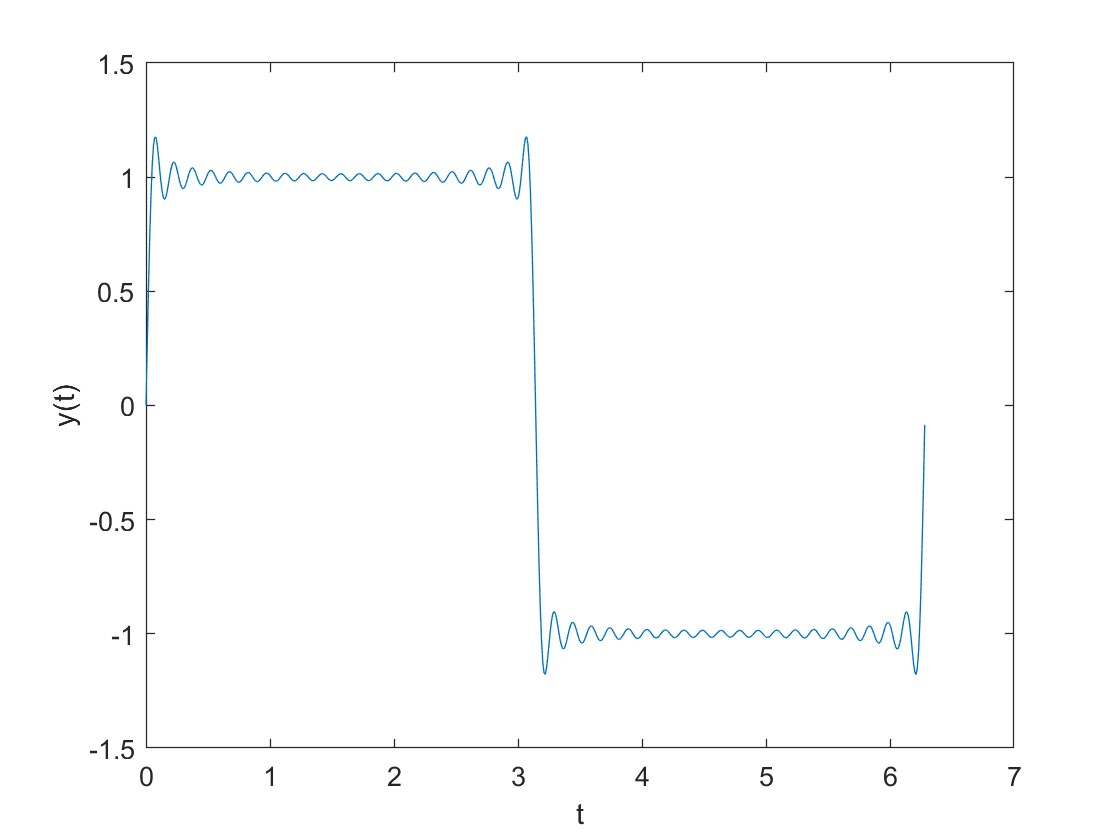
\includegraphics[width=0.5\textwidth]{gibbs}
    \caption{吉布斯现象示意图}
\end{figure}

为了直观地理解它,我们来看一个经典的例子:
\begin{align*}
    f_n(x)=
    \begin{cases}
        nx   & \text{if } 0<x\leq\frac{1}{n}        \\
        2-nx & \text{if } \frac{1}{n}<x<\frac{2}{n} \\
        0    & \text{otherwise}
    \end{cases}
\end{align*}
随n增大,$f(x)$逐点趋于0,因为对每一点$\frac{2}{n}$总能取到更小的值;但$f(x)$
的最大值永远是1。

研究傅里叶级数的渐进特性时,一个非常好用的工具是\textbf{狄利克雷核} (Dirichlet kernel):
\[D_N(t)=\sum_{k=-N}^{N}e^{ik\omega t}=1+\sum_{k=1}^{N}(e^{ik\omega t}+e^{-ik\omega t})=1+2\sum_{k=1}^{N}\cos(k\omega t)\]
它是依赖于所研究函数的周期T的,但简便起见,在符号$D_N(t)$中不体现这一点。我们可
以用等比数列求和或积化和差裂项的方法化简$D_N(t)$:
\begin{align}
    D_N(t) & =\sum_{k=-N}^{N}e^{ik\omega t}=e^{-iN\omega t}\frac{1-e^{i(2N+1)\omega t}}{1-e^{i\omega t}}                  \\
           & =\frac{e^{i(N+1)\omega t}-e^{-iN\omega t}}{e^{i\omega t}-1}\label{eq:2.8}                                    \\
    D_N(t) & =1+\sum_{k=1}^{N}(e^{ik\omega t}+e^{-ik\omega t})=1+2\sum_{k=1}^{N}\cos(k\omega t)\label{eq:2.9}             \\
           & =1+\frac{2}{\sin(\frac{\omega t}{2})}\sum_{k=1}^{N}\cos(k\omega t)\sin(\frac{\omega t}{2})                   \\
           & =1+\frac{1}{\sin(\frac{\omega t}{2})}\sum_{k=1}^{N}(\sin(k+\frac{1}{2})\omega t-\sin(k-\frac{1}{2})\omega t) \\
           & =1+\frac{\sin(N+\frac{1}{2})\omega t-\sin(\frac{\omega t}{2})}{\sin(\frac{\omega t}{2})}                     \\
           & =\frac{\sin(N+\frac{1}{2})\omega t}{\sin(\frac{\omega t}{2})}
\end{align}
这两种结果是相符的,读者可自行验证,并且可以从后一结果想象出狄利克雷核的函数图
像,它被$\pm \frac{1}{\sin(\frac{\omega t}{2})}$包络并高速振荡。根据\ref{sec:Sampling and Interpolation}
中的结果,$D_N(t)$是$\shah$函数的部分和,在$nT(n\in\mathbb{Z})$处,随$N\to\infty$,
D也趋于无穷,并在其他位置趋于0。这是又一个最大值不趋于0,但逐点趋于0的例子。函数图像如下。
\begin{figure}[htbp]
    \centering
    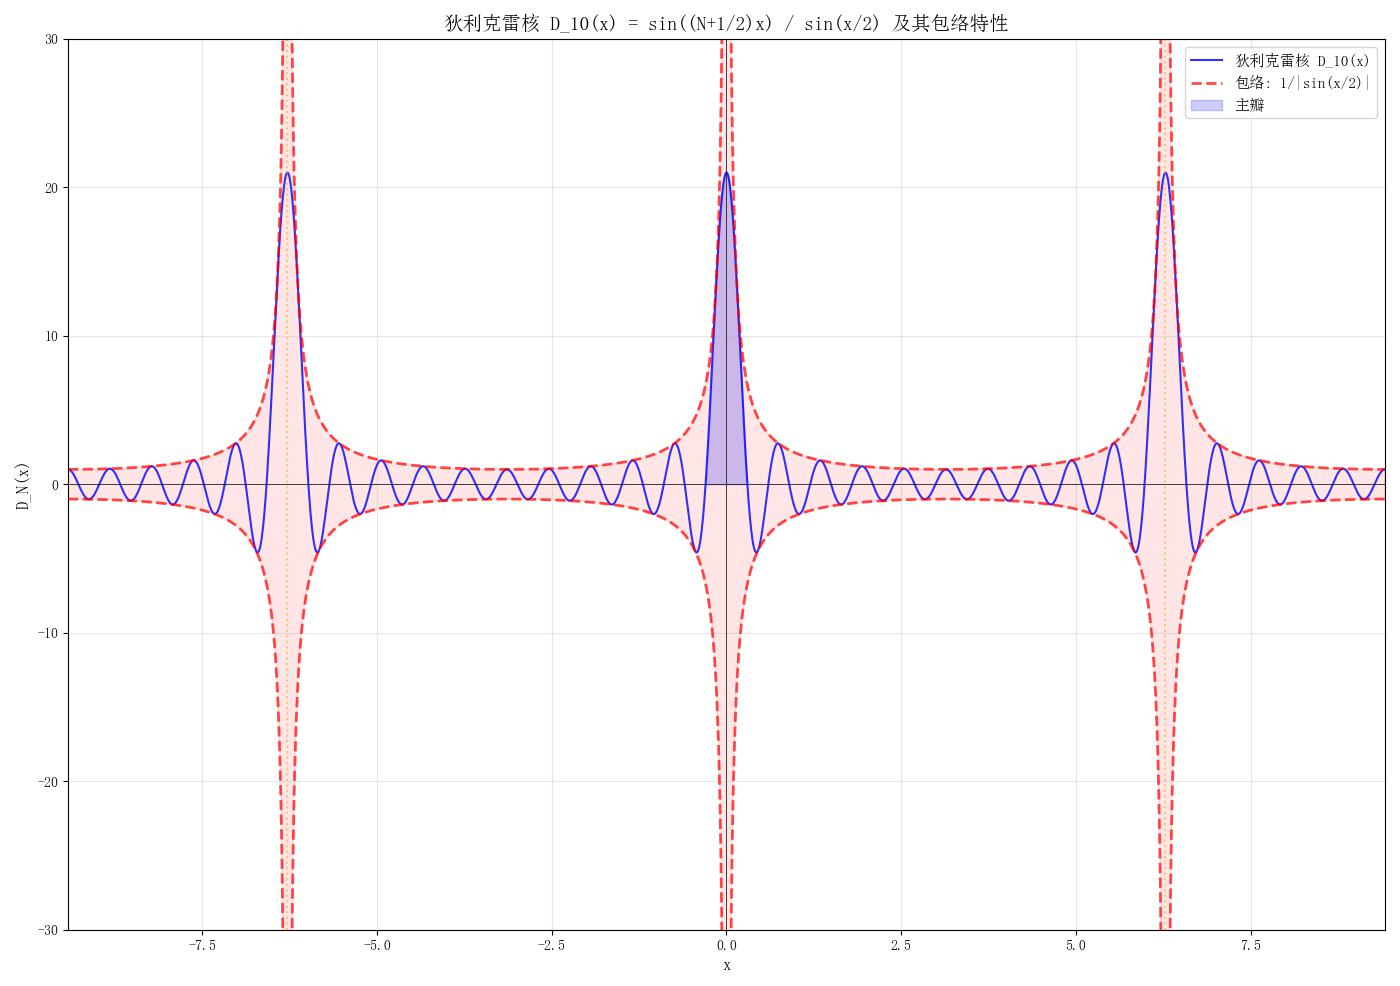
\includegraphics[width=0.7\textwidth]{Figure_3}
\end{figure}

引入狄利克雷核后,就可以用以下恒等式研究傅里叶级数的部分和:
\begin{align*}
    S_N^f(t) & =\sum_{-N}^{N}c_k e^{ik\omega t}                                                  \\
             & =\sum_{-N}^{N}(\frac{1}{T}\int_{T}f(\tau)e^{-k\omega \tau}\,d\tau) e^{ik\omega t} \\
             & =\frac{1}{T}\int_{T}f(\tau)\sum_{k=-N}^{N}e^{ik\omega (t-\tau)}\,d\tau            \\
             & =\frac{1}{T}\int_{T}f(\tau)D_N(t-\tau)\,d\tau                                     \\
             & =\frac{1}{T}\int_{T}f(t-\tau)D_N(\tau)\,d\tau\text{(变量替换)}                        \\
             & =\frac{1}{T}\int_{T}f(t+\tau)D_N(\tau)\,d\tau\text{(变量替换+周期性)}
\end{align*}

先给出两个引理。第一个引理表明狄利克雷核在半周期上积分值为$\frac{T}{2}$,在证明傅
里叶级数的逐点收敛性时将用到它。
\begin{align}
    \int_{-\frac{T}{2}}^{0}D_N(t)\,dt=\int_{0}^{\frac{T}{2}}D_N(t)\,dt=\frac{T}{2}\label{eq:2.14}
\end{align}
\begin{align*}
    \intertext{\textbf{Proof:}}
    \intertext{由公式(\ref{eq:2.9}),$D_N(t)=1+2\sum_{k=1}^{N}\cos(k\omega t)$,故}
    \int_{0}^{\frac{T}{2}}D_N(t)\,dt & =\int_{0}^{\frac{T}{2}}(1+\sum_{k=1}^{N}\cos(k\omega t))\,dt                              \\
                                     & =\frac{T}{2}+\sum_{k=1}^{N}\left.\frac{\sin(k\omega t)}{k\omega}\right|_{0}^{\frac{T}{2}} \\
                                     & =\frac{T}{2}+\frac{1}{\omega}\sum_{k=1}^{N}\frac{\sin(k\pi)}{k}=\frac{T}{2}               \\
    \intertext{$D_N(t)$是偶函数,得证。}
\end{align*}
第二个引理是\textbf{贝塞尔不等式} (Bessel's Inequality):设$ f\in L^2([0,T]),c_n=\frac{1}{T}\int_{T}f(t)e^{-ik\omega t}\,dt$,则
\begin{align}
    \sum_{-\infty}^{\infty}|c_n|^2\leq \frac{1}{T}\int_{T}|f(t)|^2\,dt\label{eq:2.15}
\end{align}
它给出了傅里叶系数平方和的上界的估计。收敛级数的通项必收敛,所以由此可以看出$c_n\to 0,n\to\infty$.
\begin{align*}
    \intertext{\textbf{Proof:}}
    |f(t)-\sum_{n=-N}^{N}c_n e^{in\omega t}|^2 & =(f(t)-\sum_{n=-N}^{N}c_n e^{in\omega t})(f(t)-\sum_{n=-N}^{N}c_n e^{in\omega t})^*                                       \\
                                               & =(f(t)-\sum_{n=-N}^{N}c_n e^{in\omega t})(f^*(t)-\sum_{n=-N}^{N}c_n e^{-in\omega t})                                      \\
                                               & =|f(t)|^2-\sum_{n=-N}^{N}(c_n^*f(t)e^{in\omega t}+c_n f^*(t)e^{-in\omega t})+\sum_{m,n=-N}^{N}c_m c_n^*e^{i(m-n)\omega t}
\end{align*}
将上式在一个周期上积分,我们知道
\[\int_{T}f(t)e^{in\omega t}\,dt=Tc_n,\int_{T}e^{i(m-n)\omega t}\,dt=\begin{cases}
        0 & \text{if }m\neq n \\
        T & \text{if }m=n
    \end{cases}\]
故\begin{align*}
      & \int_{T}|f(t)|^2\,dt-\sum_{n=-N}^{N}(c_n^*\int_{T}f(t)e^{in\omega t}\,dt+c_n \int_{T}f^*(t)e^{-in\omega t}\,dt)+\sum_{m,n=-N}^{N}c_m c_n^*\int_{T}e^{i(m-n)\omega t}\,dt \\
    = & \int_{T}|f(t)|^2\,dt-T\sum_{n=-N}^{N}(c_n^* c_n+c_n c_n^*)+T\sum_{n=-N}^{N}c_n^* c_n                                                                                     \\
    = & \int_{T}|f(t)|^2\,dt-T\sum_{n=-N}^{N}|c_n|^2
\end{align*}
这是非负函数的积分,积分值非负,即\begin{align*}
    \sum_{-\infty}^{\infty}|c_n|^2\leq \frac{1}{T}\int_{T}|f(t)|^2\,dt<\infty
\end{align*}

直接由狄利克雷条件证明逐点收敛性需要很专业的分析学工具,但我们可以适当地加强狄
利克雷条件,让$f(t)$\textbf{分段光滑} (piecewise smooth):
\[f\in PS([0,T])\Longleftrightarrow \text{除有限个点外f均可导,并且这些点是f的第一类间断点}\]
我们研究的多数函数是满足这样的性质的,并且我们将看到满足此条件会带来一些额外的
性质。此时就可以相对简单地证明逐点收敛性:
\[\lim_{N\to\infty}S_N^f(t_0)=\frac{f(t_0+)+f(t_0-)}{2}\]
\begin{align*}
    \intertext{\textbf{Proof:}}
    \text{由公式(\ref{eq:2.14}),}S_N^f(t_0)-\frac{f(t_0^+)+f(t_0^-)}{2} & =\frac{1}{T}(\int_{T}f(t_0-\tau)D_N(\tau)\,d\tau-\int_{0}^{\frac{T}{2}}f(t_0^+)D_N(\tau)\,d\tau-\int_{-\frac{T}{2}}^{0}f(t_0^-)D_N(\tau)\,d\tau) \\
                                                                     & =\frac{1}{T}(\int_{0}^{\frac{T}{2}}(f(t_0-\tau)-f(t_0^+))D_N(\tau)\,d\tau+\int_{-\frac{T}{2}}^{0}(f(t_0-\tau)-f(t_0^-))D_N(\tau)\,d\tau)         \\
    \text{由公式(\ref{eq:2.8}),}S_N^f(t_0)-\frac{f(t_0^+)+f(t_0^-)}{2}  & =\frac{1}{T}\int_{T}g(t)(e^{i(N+1)\omega t}-e^{iN\omega t})\,dt                                                                                  \\
    \text{其中}g(t)                                                    & :=\begin{cases}
                                                                             \frac{f(t_0+t)-f(t_0^-)}{e^{i\omega t}-1} & \text{if }-\frac{T}{2}<t_0<0 \\
                                                                             \frac{f(t_0+t)-f(t_0^+)}{e^{i\omega t}-1} & \text{if }0<t_0<\frac{T}{2}
                                                                         \end{cases}                                                      \\
    \text{由洛必达法则,$t\to 0$时,}\lim_{t\to 0^+}g(t)=                     & \lim_{t\to 0^+}\frac{f(t_0+t)-f(t_0^+)}{e^{i\omega t}}=\lim_{t\to 0^+}\frac{f'(t_0+t)}{ie^{i\omega t}}=\lim_{t\to 0^+}\frac{f'(t_0^+)}{i}
\end{align*}
$t\to 0^-$时同理。故g分段连续,当然是平方可积的,由定理(\ref{eq:2.15}),
$g(t)$的傅里叶系数平方和收敛,通项趋于0,$S_N^f(t_0)-\frac{f(t_0^+)+f(t_0^-)}{2}=C_{-(N+1)}-C_N\to 0$
,得证。

在分段光滑的条件下,容易得到$f'(t)$的傅里叶系数,注意微积分基本定理可以分区间使用:
\begin{equation}
    a'_n=n\omega b_n,b'_n=-n\omega a_n,c'_n=in\omega c_n
\end{equation}
以$c_n$为例:
\begin{align*}
    c'_n & =\frac{1}{T}\int_{T}f'(t)e^{-in\omega t}\,dt                                                         \\
         & =\frac{1}{T}\left.f(t)e^{-in\omega t}\right|_0^T+in\omega\int_{T}f(t)e^{-i\omega t}\,dt=in\omega c_n
\end{align*}

f的原函数F的傅里叶系数同理,并且只要\textbf{分段连续}(见\ref{sec:Fourier_Series})
即可保证f可积,但是我们必须保证F是周期函数,这要求f的直流分量为0:
\[F(t+T)-F(t)=\int_{T}f(t)dt=Tc_0=0,c_0=0\]
此时,用刚刚得到的公式(2.16)就可直接得到F的傅里叶系数:
\begin{equation}
    A_n=\frac{a_n}{n\omega},B_n=\frac{b_n}{n\omega},C_n=\frac{c_n}{in\omega}
\end{equation}

分段光滑还能够推出f的傅里叶级数\textbf{一致收敛}于f,从而可以逐项积分、逐项求
导。回顾数学分析中的魏尔斯特拉斯M判别法:对于函数项级数
$\sum_{n=1}^{\infty}f_n(x)$,如果存在正项级数$\sum_{n=1}^{\infty}M_n<\infty$
使得在区间E上$|f_n(x)|<M_n$,则$\sum_{n=1}^{\infty}f_n(x)$在E上绝对收敛且
一致收敛。对于上述命题,只需证明$\sum_{n=1}^{\infty}|c_n|<\infty$.直接应用
贝塞尔不等式是无效的,但可以通过一个小技巧完成证明:
\begin{align*}
    \text{记}c'_n\text{为f'的傅里叶系数},c'_n =in\omega c_n,                            &                                                                                \\
    \sum_{n=-\infty}^{\infty}|c_n|=   |c_0|+\sum_{n\neq 0}| \frac{c'_n}{n}|\leq & |c_0|+(\sum_{n\neq 0}\frac{1}{n^2})^{1/2}(\sum_{n\neq 0}|c'_n|^2)^{1/2}<\infty
\end{align*}
最后一步使用了柯西-施瓦兹不等式。

请读者思考:我们探究了指数形式傅里叶级数收敛的条件,对于三角函数形式的傅里叶级
数应该怎么办?

\section{分布的逼近,傅里叶反演公式}\label{sec:approach}

\section{施瓦兹函数类及其好处}\label{sec:Schwartz_Functions}

\section{与傅里叶变换有关的其他变换}\label{sec:Other_Transforms}
%正弦,余弦,拉东(?)

\end{document}
